% SuperMatics preprint. Every statement is traced to a source record in CLAIMS.md.
% Record labels R0 to R7 are defined in the introduction; the full mapping is in CLAIMS.md.
\documentclass[11pt]{article}
\usepackage[a4paper,margin=1in]{geometry}
\usepackage{amsmath,amssymb,amsthm}
\usepackage{booktabs,array}
\usepackage{xcolor}
\usepackage{tikz}
\usetikzlibrary{arrows.meta}
\usepackage{pgfplots}
\usepgfplotslibrary{groupplots}
\pgfplotsset{compat=1.16}
\usepackage[colorlinks=true,linkcolor=blue!50!black,citecolor=blue!50!black,urlcolor=blue!50!black]{hyperref}
\usepackage{xurl}
% Standard TeX stretch so the bibliography does not set underfull lines.
\setlength{\emergencystretch}{1.5em}

% ---------- evidence labels ----------
\newcommand{\PROVED}{\upshape\mdseries\textsc{Proved}}
\newcommand{\CERT}{\upshape\mdseries\textsc{Certified}}
\newcommand{\NUM}{\upshape\mdseries\textsc{Numerical}}
\newcommand{\OPEN}{\upshape\mdseries\textsc{Open}}

% ---------- notation ----------
\newcommand{\Cinf}{C_\infty}
\newcommand{\kB}{k_{\mathrm B}}
\newcommand{\Tceil}{T_{\mathrm{ceil}}}
\newcommand{\Tlin}{T_{\mathrm{lin}}}
\newcommand{\Rg}{\mathrm{ME}}
\newcommand{\dd}{\,\mathrm d}
\newcommand{\sS}{\sup\sigma S}
\newcommand{\Cgeom}{C_{\mathrm{geom}}}
\newcommand{\CLC}{C_{\mathrm{LC}}}
\newcommand{\vmax}{v_{\max}}

\newtheorem{theorem}{Theorem}[section]
\newtheorem{proposition}[theorem]{Proposition}
\newtheorem{lemma}[theorem]{Lemma}
\theoremstyle{definition}
\newtheorem{definition}[theorem]{Definition}
\newtheorem{problem}[theorem]{Open problem}
\theoremstyle{remark}
\newtheorem{remark}[theorem]{Remark}

\title{Vertex corrections and the Migdal--Eliashberg ceiling:\\ a geometric dichotomy between nested and curved Fermi surfaces}
\author{Davis Rens, SuperMatics Inc.\\\href{https://orcid.org/0000-0001-5839-5197}{ORCID 0000-0001-5839-5197}}
\newcommand{\MSPAPERDOI}{10.5281/zenodo.24410274}
\newcommand{\MSSUPPDOI}{10.5281/zenodo.24410273}
\newcommand{\MSREPOURL}{https://github.com/SuperMatics-Inc/vertex-corrections-migdal-eliashberg-ceiling}
\date{Preprint:~\href{https://doi.org/\MSPAPERDOI}{doi:\MSPAPERDOI}\\
Supplementary records:~\href{https://doi.org/\MSSUPPDOI}{doi:\MSSUPPDOI}\\
Source:~\url{\MSREPOURL}}

\begin{document}
\maketitle

\begin{abstract}
The phonon-only scalar Migdal--Eliashberg (ME) equations on the positive reflected normal branches specified below have the ceiling $\kB\Tlin<\Cinf\sqrt{AM}$, where $A$ is the relative height of the electronic density of states and $M=\int\Omega^2\dd\lambda(\Omega)$ is the phonon spectral moment. The exact coefficient $\Cinf$ rounds to $0.18272624777232952$ \cite{RensScalar}. We ask whether this ceiling survives addition of the first crossed skeleton to the rainbow self-energy, and the answer we obtain is a geometric dichotomy rather than a single uniform bound.

On the negative side, bounded density of states, a constant transfer $V_j=K_j/N_0$ and a fixed bare chemical potential are not sufficient. On a one-dimensional band, and on the parallel flat sheets of a two-dimensional band, the crossed skeleton has a nonvanishing limit as $\Omega/W\to0$: three of the four sheet combinations satisfy linear energy conservation, the fourth is separated by the full bandwidth, and the crossed channels reduce to two exact Cauchy residues. The linearized pairing operator of that limit is self-adjoint and its top eigenvalue crosses unity at $\lambda=4,6,8$, with Richardson values $1.004245$, $1.013678$, $1.014628$, so the onset lies $0.9\%$ to $6.5\%$ above the ceiling. The crossing of that limit is numerical. At two fixed discretisation points the truncated finite-band equations are now certified: at $N_k=24$, $N_w=12$, $\lambda=8$, $\eta=1$, $\mu_0=-2/5$ and $m=1/100$ and $1/200$, the normal branch is the unique fixed point of the truncated map in the sup-norm ball of radius $10^{-12}$, and the linearised gap operator stays above unity over the whole enclosing box, with the certified bound clearing a threshold of $1+\theta$, $\theta=5\times10^{-3}$, by at least $7.97\times10^{-4}$ and $1.49\times10^{-2}$. That certificate governs a finite discretised model, not the continuum operator. The rainbow-only column of the same lattices stays below unity, at $0.9801$ and $0.9945$, so the crossing is a vertex effect, but that comparison is numerical. The band is nested, its $2k_F$ charge response is strongly enhanced, and the branch used is therefore not a physical ground state.

On the positive side, the small-$x$ exclusion proved here for a spherical band is a special case of a statement about curvature. For every $d\ge2$, a compact $C^2$ dispersion whose energy collars are strictly convex, with nondegenerate pocket tangencies, satisfies a uniform three-line strip overlap bound in which a coarea estimate along the collars replaces the spherical joint density. A layer-cake reduction turns that bound into a relative crossed correction of order $x(1+\log_+(1/x))^{4}$ in $d=2$ and $x(1+\log_+(1/x))^{3}$ in $d\ge3$, and the crossed form is then a relative $o(1)$ perturbation of the ME form in the adiabatic window, on any sign-preserving normal branch with the stated bounds. The all-$x$ Young-ball closure of the pointwise criterion $AR\le1/9$ survives unchanged for a constant transfer and a particle-hole-even density of states.

The earlier results remain: an explicit inflation for a local flat band, stability above an inflated threshold in the spherical window, an onset bound strictly below the ceiling for $A\lambda\le1/26^2$, continuum estimates and finite arithmetic certificates for the spherical Einstein model at $1/9\le\lambda\le2$, and three grid-refined numerical pairing roots in a finite lattice. What remains open is narrower than before: intermediate $x$ at $\lambda\ge1/9$ without spherical symmetry, existence of the normal branch without particle-hole symmetry, the Matsubara tail and the continuum and adiabatic limits of the flat-sheet crossing, which is certified so far at two discretisation points, and degenerate tangencies.
\end{abstract}

\tableofcontents

%--------------------------------------------------------------------
\section{Introduction and question}\label{sec:intro}

The ME comparison used here is scalar and phonon-only, with a momentum- and electronic-energy-independent vertex and the same nonnegative transfer in the normal and pairing channels. It assumes positive reflected normal widths, nonzero finite phonon mass and second moment, and finite DOS height relative to a positive reference $N_0$. For even-frequency singlet pairing we write
\begin{equation}\label{eq:ceiling}
\Tceil=\frac{\Cinf\sqrt{A\,M}}{\kB},\qquad \Cinf=\frac{\sqrt{g(2)}}{2\pi},
\end{equation}
where $g(2)$ is the spectral top of the soft scalar $\gamma=2$ operator. The exact coefficient is used in the guards; $0.18272624777232952$ is rounded and exceeds the certified upper endpoint $0.1827262477723295176168720$ (record R0, certified endpoint). The scalar result is \cite{RensScalar}, on the conjectures of Kiessling, Altshuler and Yuzbashyan \cite{KAYGamma,KAY}; related work and formalisations include \cite{Kondratev,Siraj,KumarGSI}. The finite-DOS extensions are \PROVED\ (computer-assisted). Case~(a) uses a common real shift at fixed temperature, centered for even DOS when the real integral converges or has a symmetric principal-value prescription on infinite bands. Case~(e) uses a self-consistent asymmetric branch with the relative real equation defined in ordinary Matsubara order. We do not combine these extensions with each other and do not assert an anisotropic or Coulomb-inclusive theorem. For other phonon-mediated bounds see \cite{MoussaCohen,EsterlisBound}.

Migdal's approximation neglects vertex corrections, and the first of them is the crossed (vertex-corrected) self-energy diagram. Full-bandwidth treatments beyond Migdal exist \cite{Schrodi}, and the vertex expansion has an extensive literature, for example \cite{Miller,Paci,GrimaldiI,GrimaldiII,GrimaldiScattoni,ChubukovVertex}. Recent work examines where Migdal--Eliashberg theory breaks down in Holstein-type models, through quantum Monte Carlo \cite{EsterlisBreakdown}, polaron and bipolaron formation \cite{ChubukovVertex,ChubukovPolaron}, and, for a specific material, a calculation that includes the leading vertex correction \cite{Mishra}. The question addressed here is narrower.

\begin{quote}\emph{Does the proved ME ceiling \eqref{eq:ceiling} survive the first vertex correction?}\end{quote}

Here ``survive'' refers to the upper linear pairing boundary on a named normal branch where it exists, for rainbow plus first crossed with bare phonons, fixed chemical potential and no Coulomb term. Most bounds use the regular branch; Theorem~\ref{thm:V1} applies to any solution with the specified centering and widths.

\paragraph{What is shown.}
The question above does not have a single answer, and the central result of this version is that it splits along the geometry of the energy surfaces. Bounded density of states, a constant transfer and a fixed chemical potential do not bound the crossed skeleton on nested sheets, and strict convexity of the energy collars does bound it on curved ones.
\begin{itemize}
\item \PROVED\ On a one-dimensional band, and on the parallel flat sheets of a two-dimensional band, the crossed skeleton has an $O(1)$ limit as $\Omega_{\max}/W\to0$. Three of the four sheet combinations satisfy linear energy conservation, the fourth is separated by the bandwidth, and the two crossed channels reduce to the exact residues $I_1$ and $I_{23}$ (Theorem~\ref{thm:flat}). The first crossed correction does not vanish as $m\to0$ on these bands.
\item \NUM\ and \CERT\ (padded binary64) at two fixed parameters: the self-adjoint pairing operator of the crossed limit has top eigenvalue $1.004245$, $1.013678$, $1.014628$ after Richardson extrapolation at $\lambda=4,6,8$, so the linear onset lies $0.9\%$ to $6.5\%$ above the ceiling (Proposition~\ref{prop:flatcross}). The band is nested and its static $2k_F$ charge response is strongly enhanced, so this is a statement about the truncated equations and not about a ground state.
\item \CERT\ at two discretisation points of the truncated band. At $N_k=24$, $N_w=12$, $\lambda=8$, $\eta=1$, $\mu_0=-2/5$ and phonon-mass ratio $m=1/100$ or $1/200$, the normal-state map of the finite model has exactly one fixed point in the sup-norm ball of radius $10^{-12}$, by an outward-rounded Krawczyk test, and the linearised gap operator is at least $1.00579751250$ or $1.01993371122$ at every point of the enclosing box (Theorem~\ref{thm:C}). Ten deliberately broken variants are refused, both bounds are reproduced at 400-bit working precision, and a separately written checker reproduces both the fixed point and the crossing for both models. The statement concerns the finite discretised equations. The Matsubara tail, the continuum momentum limit and the adiabatic limit stay \NUM, and so does the comparison with the rainbow kernel.
\item \PROVED\ For every $d\ge2$, strict convexity of the energy collars, a uniform lower bound on the Fermi velocity and nondegenerate pocket tangencies give the three-line strip overlap bound used before only in spherical or balanced geometry (Lemma~\ref{lem:coarea}). A layer-cake reduction then makes the crossed form a relative $o(1)$ correction to the ME form in the small-$x$ window (Lemma~\ref{lem:layercake}, Theorem~\ref{thm:curved}). The spherical small-$x$ exclusion of Theorem~\ref{thm:V3a} is the spherical special case.
\item \PROVED\ A local crossed skeleton with flat DOS obeys the ceiling inflated by a factor that tends to $1$ as $\Omega_{\max}/W\to0$ at fixed $\lambda$ (Theorem~\ref{thm:V1}), and two tempting estimates are shown to be false (Proposition~\ref{prop:obstruction}, Theorem~\ref{thm:V2}).
\item \PROVED\ The spherical estimate excludes instability within $x\le x_*$ above an inflated threshold (Theorem~\ref{thm:V3a}). The pointwise Young-ball criterion $AR(T)\le1/9$ gives stability above $\tau_Y$ if $A\lambda<1/9$, and an onset bound strictly below the ceiling if $A\lambda\le1/26^2$ (Theorem~\ref{thm:V3b}). The overlap theorem gives the uninflated bound under a sufficient guard (Theorem~\ref{thm:B2}).
\item \PROVED\ and \CERT\ for the spherical Einstein model at $1/9\le\lambda\le2$, two full-coupling windows, a weak edge interval, and finite grids (Theorem~\ref{thm:V4} and Propositions~\ref{prop:V4grid},~\ref{prop:V4static}). The grid labels certify nodes, not a continuum of parameters.
\item \NUM\ Three grid-refined homogeneous-branch pairing roots below the ceiling at fixed density in a finite-DOS lattice (Section~\ref{sec:lattice}); the largest onset over all branches is unknown.
\end{itemize}

\paragraph{What is not claimed.} We do not claim that vertex corrections preserve or violate the ceiling in general, or that the local conserving crossed treatment is new \cite{Miller}. The flat-sheet result does not claim that any material is superconducting, and it does not claim that pairing wins against the charge or Peierls instability of that band; the opposite is indicated by the enhancement reported with it. The curved-surface result does not claim that the crossed skeleton can lower the onset, only that in the adiabatic window it cannot raise it by more than a relative amount that vanishes with $x$. An earlier \NUM\ van Hove model gave $134.27$~K against a rounded $A=1$ scalar reference of $129.85$~K on a $24\times24$ grid with 24 positive Matsubara frequencies. The momentum grid is not converged and the DOS has $A=\infty$, so the reference is not its ceiling (Section~\ref{sec:lattice}). Theorem~\ref{thm:C} is a statement about a finite discretised model at two parameter points: it does not bound the continuum operator, it carries no Matsubara tail, and its certified clearance of the threshold at $m=1/100$, about $8\times10^{-4}$ above $1+\theta$, is a discretisation-scale margin rather than a physically resolved one. Nothing here is a measurement or a prediction of a material's $T_c$.

\paragraph{Version 2 note.} This version adds two results and rewrites what follows from them. The released first version left the universal onset question open in both directions, with neither a uniform bound for the crossed skeleton nor a counterexample. The added results settle one direction on nested sheets and widen the other direction from a spherical model to a curvature condition: Theorem~\ref{thm:flat} and Propositions~\ref{prop:flatcross} and~\ref{prop:flatcert} supply the counterexample (analytic scaling limit, numerical crossing, and padded-binary64 finite-band lower bounds) and Lemmas~\ref{lem:coarea},~\ref{lem:layercake} and Theorem~\ref{thm:curved} supply the bound. Nothing asserted in the first version is withdrawn. Theorem~\ref{thm:V3a} keeps its statement and its proof and is now understood as the spherical instance of Theorem~\ref{thm:curved}; Theorem~\ref{thm:V3b} keeps its statement and appears again as part (1) of Theorem~\ref{thm:curved}, where its two extra hypotheses are shown to be necessary for an all-$x$ closure. The statement of Theorem~\ref{thm:V2} that the universal onset question was open, and the open problem of Section~\ref{sec:open} that carried the same name, are superseded: the question is now posed as four separate problems, and the first of them, the intermediate-$x$ window at $\lambda\ge1/9$, is where the remaining difficulty sits.

\paragraph{Version 3 note.} This version adds one result and changes the status of one statement of the previous version. The finite-band crossing was certified there only by a padded binary64 Rayleigh quotient of a computed normal solution, which left the existence and uniqueness of that normal solution as the first of three open gaps. Section~\ref{sec:certified} now proves, in ball arithmetic, that the truncated model at $N_k=24$, $N_w=12$, $\lambda=8$, $\eta=1$, $\mu_0=-2/5$ and $m=1/100$ and $m=1/200$ has exactly one fixed point in the sup-norm ball of radius $10^{-12}$ and that its linearised gap operator exceeds unity over the whole enclosing box (Theorem~\ref{thm:C}); ten deliberately broken variants of the certificate are refused, and a second, separately written checker reproduces both the fixed point and the crossing for both models. Nothing asserted in the earlier versions is withdrawn. Proposition~\ref{prop:flatcross} keeps its \NUM\ label for the crossing of the scaling limit, Proposition~\ref{prop:flatcert} keeps its padded binary64 label and its scope at $m=0.005$ and $0.008$ with momentum grids of a few thousand points, part~(V) of Theorem~\ref{thm:C} keeps its \NUM\ label for vertex-decisiveness, and the Matsubara tail and the two continuum limits of Open problem~\ref{prob:flatcert} remain open. What changes is that the first of those gaps is now closed for a smaller truncation, so the certification problem is posed at two discretisation points that are proved and at the limits that are not.

\paragraph{Supplementary records.} The full proofs, replay scripts and certificate logs accompany this preprint as supplementary material and are grouped as R0 to R7: R0 the scalar ceiling, R1 the local crossed skeleton, R2 the signed momentum-resolved form together with its formalised algebra, R3 the spherical onset estimates, R4 the spherical Einstein gap and grid, R5 the finite lattice, R6 the flat-sheet limit and the curved-surface bound added in version 2, and R7 the certified fixed point and crossing of the finite two-flat-sheet model added in this version. Each statement below names the record, section and line that prove it. Numerical work is reproduced by the replay supplement described in Section~\ref{sec:verification}.

\paragraph{Plan.} Section~\ref{sec:model} defines the model. Section~\ref{sec:results} states the earlier results with exact hypotheses and displays their coverage in the $(x,\lambda)$ plane. Section~\ref{sec:flat} states the flat-sheet result added in the second version together with the certificate added in this one (Section~\ref{sec:certified}), Section~\ref{sec:curved} states the curved-surface bound, Section~\ref{sec:proofs} gives proof sketches and points to the full proofs in the records R1 to R7, Section~\ref{sec:verification} describes the computer-assisted and Lean verification and its limits, Section~\ref{sec:lattice} the finite-lattice numerics, Section~\ref{sec:conclusions} the dichotomy and its scope, and Section~\ref{sec:open} what remains open.

%--------------------------------------------------------------------
\section{Model}\label{sec:model}

\subsection{Notation and the first crossed skeleton}

Use energy units for $\Omega$ and $\tau=\kB T$. Set $\nu=\pi\tau$, $\omega_n=(2n+1)\nu$ and $x=\nu/W$, with $W$ the band half-width. For the crossed bounds take a nonnegative measure $\dd\lambda(\Omega)$ of finite positive mass $\lambda$ on $(0,\Omega_{\max}]$:
\begin{equation}\label{eq:moments}
K_j=\int\frac{\Omega^2}{\Omega^2+(2\nu j)^2}\dd\lambda(\Omega),\quad K_0=\lambda,\quad M=\int\Omega^2\dd\lambda,\quad R=\sum_{j\in\mathbb Z}K_j,\quad L=\sum_{j\ge1}K_j,
\end{equation}
with $m=\Omega_{\max}/W$ and $\rho=m\sqrt\lambda$. The Einstein measure is a single atom of mass $\lambda$ at $\Omega$, and $M=\lambda\Omega^2$. The finite DOS ratio is $A=\operatorname*{ess\,sup}_\xi N(\xi)/N_0$ with $0<N_0=N(0)<\infty$. Momentum and its DOS pushforward are normalized per spin to one state (per cell for lattice bands); Matsubara sums use counting measure. Write $\eta=T/\Tceil$.

\begin{definition}[First crossed skeleton]\label{def:skeleton}
The Nambu self-energy is the sum of the rainbow term and the crossed term,
\begin{equation}\label{eq:skeleton}
\Sigma_p=\tau\sum_{s}V_{p-s}\,\sigma_3G_s\sigma_3\;+\;\tau^2\sum_{s,t}V_{s}V_{t}\;\sigma_3G_a\sigma_3G_b\sigma_3G_c\sigma_3,
\end{equation}
with $a=p-s$, $b=p-s-t$, $c=p-t$. Each four-label carries momentum and Matsubara index, and its sum includes momentum integration. We use bare phonons, fixed chemical potential, no Coulomb term and even-frequency singlet pairing. For a constant spatial transfer, $V_j=K_j/N_0$.
\end{definition}

In the local version (Theorem~\ref{thm:V1}) each line is integrated separately against the DOS, at fixed half-filled chemical potential with a constant Hartree offset absorbed. The momentum-resolved version imposes $a+c-b=p$. Before normal-state elimination its real anomalous insertions at $a,b,c$ have coefficients $\operatorname{Re}(z_bz_c)$, $\operatorname{Re}(z_a\overline{z_c})$ and $\operatorname{Re}(z_az_b)$, respectively. The alternating square arises in the eliminated form, not from an overall minus sign on the raw middle insertion.

\subsection{The spherical overlap model}

\begin{definition}[Spherical overlap model]\label{def:spherical}
Let $D\subset\mathbb R^3$ be the unit ball with Lebesgue measure divided by $\mathrm{vol}(D)$, and set all lines to zero outside $D$. The dispersion is $\xi(k)=W(2|k|^3-1)$ on $D$, giving a flat DOS on $[-W,W]$, $N_0=1/(2W)$, $A=1$ and $E_F=W$. The transfer is $V_j=K_j/N_0$. The spectrum is specified separately: Theorem~\ref{thm:V2}(iii)--(iv) and Theorem~\ref{thm:V4} are Einstein, while Theorem~\ref{thm:V3a} and the uniform Theorem~\ref{thm:B2} statement permit general spectra. Theorem~\ref{thm:V3a} also treats a balanced spectator circle.
\end{definition}

For the three-line phase space at fixed external momentum $k$ with $K=|k|>0$, the joint measure in $\dd\xi_a\dd\xi_b\dd\xi_c$ is, almost everywhere and with no dropped factor, the product of the envelope
\begin{equation}\label{eq:joint}
\frac{\dd\xi_a\dd\xi_b\dd\xi_c}{48\,W^3R_aR_bR_c},\qquad R_i=\Big(\tfrac{1+\xi_i/W}{2}\Big)^{1/3},
\end{equation}
and the angular factor
\[
\Theta=\frac{\operatorname{length}\big([|R_a-K|,R_a+K]\cap[|R_b-R_c|,R_b+R_c]\big)}{2K}\le1 .
\]
The measure is thereby equal to that product, not merely bounded by it: $\Theta$ is the exact normalized angular-overlap factor at fixed radii, and the fold estimates below use this exact joint density. At $K=0$ the law takes a different form, and there the envelope~\eqref{eq:joint} is used only as an upper bound. The projection is a model choice, not a lattice approximation or a fit to a material.

\subsection{The regular branch and the onset}

\begin{definition}[Regular branch, onset]\label{def:regular}
The \emph{regular branch} is the normal solution continued from zero interaction at the same temperature, where justified by a contraction. It is not an arbitrary positive-width solution. For the self-adjoint linearised pairing kernel $B$, strict instability means $\sup\sigma(B)>1$, equality is marginal, and strict stability means $\sup\sigma(B)<1$. We use $\Tlin$ for the supremum of temperatures with $\sup\sigma(B)\ge1$ on the named branch where it exists, and zero for an empty set. Strict stability excludes either convention for counting the marginal point. The relevant form is congruent to $I-B$; negative eigenvalues below $-1$ do not signal a pairing instability.
\end{definition}

Existence and uniqueness of other branches, real-axis causality and competing orders are not asserted anywhere below. We also stress what a statement of the form $\kB\Tlin\le\Cinf\sqrt{AM}$ is: a property of the linearised, truncated equations on a named branch, not a statement about the many-body transition temperature.

\subsection{Labels}

\PROVED\ denotes a complete analytic proof that has passed an independent review recorded with the supplementary material, or an exact rational argument. \CERT\ denotes a finite arithmetic enclosure: the peak guards are checked by exact rational and interval calculations, while the signed-tube and radial parts use padded binary64 under the assumptions in Section~\ref{sec:verification}. Record R7 uses \CERT\ in a stronger sense: arbitrary-precision ball and directed-rounding interval arithmetic, a second separately written checker, and guarded broken variants, with binary64 used only to select starting data. \NUM\ denotes a computation without such an enclosure.

%--------------------------------------------------------------------
\section{Results}\label{sec:results}

In every theorem the hypothesis list is part of the statement. Constants such as $2^{-80}B^{-8}$ are sufficient, not sharp.

\subsection{A local crossed skeleton}

\begin{theorem}[Local crossed skeleton, flat DOS]\label{thm:V1}\hfill\PROVED\\
Take a flat DOS on $[-W,W]$ ($A=1$), the local first crossed skeleton and even-frequency singlet pairing. For any centered particle--hole-symmetric normal solution ($\chi_n=0$) with positive reflected widths, the pairing stability estimate gives
\begin{equation}\label{eq:V1}
\kB\Tlin\;\le\;\Cinf\sqrt{AM}\,\Big[1+30\big((1+\lambda)\rho+\rho^2\big)\Big].
\end{equation}
The bound does not require a regular branch or the existence guard. If $(1+\lambda)\rho\le1/100$, a centered positive-width solution exists pointwise for every $\tau\in[\Cinf\sqrt M,\,2\Cinf\sqrt M]$. At fixed finite $\lambda$, the uninflated ceiling holds if $\epsilon=30[(1+\lambda)\rho+\rho^2]<\delta_\lambda$, where $\delta_\lambda=1-\lambda h((2\pi\Cinf\sqrt\lambda)^{-1})>0$ and $h$ is the scalar Einstein spectral top per unit coupling.
\end{theorem}

The inflation need not be uniformly small; the sufficient regime is $(1+\lambda)\rho\ll1$. Neither branch selection, uniqueness nor real-axis causality is asserted. The vertex-specific content is the cancellation in Lemma~\ref{lem:local}. Miller et al.\ give an earlier local conserving treatment \cite{Miller}; Paci et al.\ compute the local-vertex onset with a half-filled constant DOS \cite{Paci}.

\begin{proposition}[Two estimates that fail]\label{prop:obstruction}\hfill\PROVED\\
At fixed positive $\lambda$ and $\tau=\Omega$, the dynamic triangle at zero spatial transfer and frequency pair $(-1,0)$ tends as $m\to0$ to $\lambda$ for bare and $\lambda/(1+\lambda)$ for ME-dressed flat-band lines. In the simple-cubic example only the bare pointwise limit $\lambda$ is established. For $m\le1/20$, the norm of the absolute Cooper-weighted frequency block of one bare flat-band end insertion is at least $\lambda K_1\arctan(1/16)/(2\pi)$, with $K_1=\lambda/(1+4\pi^2)$.
\end{proposition}

Continuity in spatial transfer rules out an essential-supremum $O(\lambda m)$ triangle estimate for these examples. A termwise absolute bound vanishing with $m$ cannot hold uniformly for the specified bare blocks. Neither result bounds the fully crossed self-consistent operator or the sum of signed terms.

\subsection{Signed crossed form in a momentum-resolved model}

\begin{theorem}[Signed form, forward limit, obstruction, overlap window]\label{thm:V2}\hfill\PROVED, with scope as stated\\
Let the first crossed skeleton be momentum resolved with Einstein phonons and $\Cinf$ as above.
\begin{enumerate}
\item[(i)] \emph{Ultranarrow forward limit.} On $[-\pi,\pi)$ take $\xi=W(2|k|/\pi-1)$ ($A=1$, $E_F=W$, $v_F=2W/\pi$), $M=\lambda\Omega^2$, fixed finite positive Fermi-surface coupling $\lambda$, and $V_j(q)=4\lambda W\,\mathbf1_{|q|\le q_c}\Omega^2/[\Omega^2+(2\nu j)^2]$ with $0<q_c<\pi$. If $v_Fq_c=o(\Omega)$, the regular branch is stable for every $\tau$ above any fixed positive fraction of $\sqrt\lambda\,\Omega$ as $m\to0$.
\item[(ii)] \emph{A negative crossed contribution need not vanish.} Even at the exact ceiling, take the same forward model at fixed $\lambda=2^{32}$, $\tau=\Cinf\sqrt\lambda\,\Omega$, and $v_Fq_c=(\delta/\lambda)\nu$. Thus $\lambda\Omega/E_F\to0$ as $m\to0$. Write $B_0=\int V_0=2\lambda v_Fq_c$, $r_0=B_0/(\pi^2\tau)$ and $k_1=K_1/\lambda$. For the localized trial use $\delta=2^{-16}$: the margin is $55/262144>1/8192$ and $F_X/Q_0\le-r_0^2/16384$. For the momentum-independent trial gap fix sufficiently small $\delta>0$ before taking small $m$: $F_X/Q_0\le-r_0^2k_1/128$, with $k_1<1/1000$. Both families obey $F\ge(9/32)Q_0$ for all admissible trials, so neither is an onset counterexample.
\item[(iii)] \emph{Overlap window.} In the spherical overlap model of Definition~\ref{def:spherical} with Einstein coupling $\lambda$, there is $t_0(\lambda)<\Cinf\sqrt\lambda$ and $x_\lambda>0$ such that the regular branch has no even-frequency singlet onset for $t_0(\lambda)\,\Omega\le\tau\le x_\lambda W/\pi$ (the window is non-empty for $\Omega/W$ small enough), and $|F_X|/Q_0=O_\lambda\big((\tau/W)[1+\log(W/\tau)]^3\big)$ as $\tau/W\to0$. The result is qualitative in $\lambda$ and not uniform as $\lambda\to\infty$.
\item[(iv)] \emph{Weak coupling in the projected spherical Einstein model of (iii).} For $0<\lambda\le2^{-20}$ the regular branch is stable at every $\tau\ge\sqrt\lambda\,\Omega/8$, without restriction on $m$. Hence $\tau_{\rm lin}\le\sqrt\lambda\,\Omega/8<\Cinf\sqrt M$.
\end{enumerate}
The universal onset statement of the first version is not settled by this theorem; Section~\ref{sec:flat} and Section~\ref{sec:curved} replace it by the dichotomy stated in this version.
\end{theorem}

Part~(ii) is the reason the proofs below cannot treat the crossed term as a small perturbation of the ME gap. The Lean-checked finite algebra behind parts of this theorem is listed in Section~\ref{sec:verification}.

\subsection{Spherical band and the Young-ball regime}

\begin{theorem}[Signed spherical window]\label{thm:V3a}\hfill\PROVED\\
Take the spherical band with a general spectrum as in~\eqref{eq:moments}, or extend it to $D\times\mathbb T$ with normalized Haar measure on the circle, $\xi(k,\theta)=\xi(k)$ and $V_j(q,q_\theta)=K_jv(q_\theta)/N_0$. Here $v$ is even, nonnegative and of mean one, and $\|v-1\|_1\le1/(16B)$. Set $B\ge\max(1,\lambda+3\sqrt\lambda)$ and $x_*=2^{-80}B^{-8}$. For $\tau\ge\tau_c=\Cinf\sqrt M$ and $0<x\le x_*$ the regular branch exists and the pairing form satisfies
\begin{equation}\label{eq:V3a}
F[y]\;\ge\;\big[1-\sS(1)-C_0x\big]\,Q_0[\bar y]+\tfrac38\,Q_0[y_\perp],\qquad C_0=13000\,B^4,
\end{equation}
where $\bar y_n$ is the mean over all momentum variables in the probability measure proportional to $|Q_n|$, and $y_\perp=y-\bar y$. Within $0<x\le x_*$, stability holds for $T\ge\Tceil(1+52000\,B^4\rho)$. The constants are sufficient, not sharp, and not uniform as $B\to\infty$.
\end{theorem}

\noindent\emph{Relation to the new curved-surface result.} The statement and proof of Theorem~\ref{thm:V3a} are unchanged in this version. It is now the rotationally symmetric instance of part (2) of Theorem~\ref{thm:curved}: the coarea bound of Lemma~\ref{lem:coarea} reduces to the spherical joint density and its constants, so the spherical exclusion is neither withdrawn nor weakened, only narrowed to the case where the extra symmetry was doing no work.

\begin{theorem}[Young-ball criterion and weak-coupling onset bound]\label{thm:V3b}\hfill\PROVED\\
Use a constant spatial transfer on an inversion-invariant projected continuum domain or additive momentum group with Haar measure, with $\xi(-k)=\xi(k)$ almost everywhere and an even normalized marginal DOS bounded by $AN_0$. At any $\tau>0$ such that $r=AR(\tau)\le1/9$, contraction gives the unique regular solution within $\|\Sigma\|_\infty\le\nu/3$, and pairing has absolute Schur bound strictly below one. The criterion holds at every $\tau\ge\tau_Y$ if $A\lambda<1/9$, yielding
\begin{equation}\label{eq:V3b}
\kB\Tlin\le\tau_Y=\frac{9\,A\,M_1}{2\,(1-9A\lambda)},\qquad M_1=\int\Omega\dd\lambda(\Omega),
\end{equation}
and for $A\lambda\le1/26^2$ one has $\tau_Y<\tfrac{9}{50}\sqrt{AM}<\Cinf\sqrt{AM}$, with no adiabatic assumption. This does not exclude pairing at temperatures below $\tau_Y$.
\end{theorem}

\begin{theorem}[Overlap of the two regimes]\label{thm:B2}\hfill\PROVED\\
For fixed Einstein $0<\lambda<1/9$ and sufficiently small $\Omega/W$, the spherical window of Theorem~\ref{thm:V2}(iii) joins the Young-ball regime to give stability for every $\tau\ge t_0(\lambda)\Omega$, with $t_0(\lambda)<\Cinf\sqrt\lambda$. For general spectra on the sphere and its balanced extension the low-$x$ estimate is instead Theorem~\ref{thm:V3a}. For $0<\lambda\le\Lambda<1/9$, a sufficient guard for the uniform uninflated ceiling is
\begin{equation}\label{eq:B2}
\rho<\frac{x_h}{\pi}\sqrt{12\Big(\frac19-\Lambda\Big)},
\end{equation}
with $\delta_*=\inf_{\lambda\le\Lambda}\delta_\lambda>0$, $B=1+\Lambda+3\sqrt\Lambda$ and $x_h=\min(x_*,\delta_*/(2C_0))$. The two contraction regimes overlap on $\max(x_c,x_Y)<x<x_h$, where $x_c=\pi\tau_c/W$ and $x_Y=\pi\rho/\sqrt{12(1/9-\Lambda)}$. On that branch $\tau_{\rm lin}\le\tau_c$. The result is not uniform in unbounded coupling and contains no claim of a crossing or of a universal ceiling.
\end{theorem}

\noindent\OPEN: marginal DOS control alone gives neither the joint-density regularity nor the balanced variance estimate. (Sections~\ref{sec:flat} and~\ref{sec:curved} show that bounded DOS alone fails on nested sheets and that strict convexity replaces the spherical joint density at small $x$.) The Young-ball high-temperature conclusion for $A\lambda<1/9$ does not address larger couplings, and the small-$x$ estimates deteriorate with growing $\lambda$.

\subsection{Spherical Einstein model at \texorpdfstring{$1/9\le\lambda\le2$}{couplings from 1/9 to 2}}

All statements here concern the projected spherical Einstein band with $A=1$, fixed chemical potential and the rainbow plus first crossed skeleton. Stability results concern the regular continuation from zero coupling, with the full Matsubara line and all allowed momentum sectors, not just radial trial gaps. The record R4 has been independently reviewed, and that review covers both the continuum and grid claims and qualifies the arithmetic trust base in Section~\ref{sec:verification}.

\begin{theorem}[Continuum windows and weak edge]\label{thm:V4}
\noindent\PROVED\ (analytic estimates, with separate checks of the constants).
\begin{enumerate}
\item[(i)] \emph{Static-transfer limit.} As $\Omega/W\to0$ at fixed $x$ and $\lambda$ (with $W=1$ and $g=2\lambda x/\pi$), the rainbow and first crossed normal terms become, on each Matsubara block, $\Sigma_n=g\!\int_D z_n\,\dd\mu+g^2(z_n*z_n*z_n)|_D$. Here $*$ is the normalized spatial convolution of zero-extended lines. Writing $z_n=r_n-iQ_n$, the unsymmetrized vertex $g+g^2(3\,r_n*r_n-Q_n*Q_n)$ enters the block kernel between the weights $|z_n(p)|$ and $|z_n(k)|$. The negative $Q_n*Q_n$ term is kept. The Ward identity gives a conditional positivity criterion: the unsymmetrized vertex is pointwise nonnegative if $g\|z_n\|_2^2\le1$ on every block, which is an assumption about the branch and not a consequence of the theorem. The limit is $\eta\to\infty$, not the slice $\eta=1$.
\item[(ii)] \emph{Small $x$.} For $0<x\le2^{-40}$, $1/9\le\lambda\le2$ and $\eta\ge1$, the regular branch exists with pairing gap $>0.00807313$. This uses the absolute spatial overlap estimate, not the signed bound in Theorem~\ref{thm:V3a}.
\item[(iii)] \emph{Large $x$.} For $x\ge19/2$ on the same coupling and temperature-ratio range, a contraction from zero coupling gives pairing spectral top $<0.70468692$.
\item[(iv)] \emph{Weak edge.} If $R\le3/25$, the regular branch has pairing spectral top $\le0.78467306$. In the static model this covers all $x>0$ for $1/9\le\lambda\le3/25$. In the finite Einstein model with $1/9\le\lambda\le7/60$, it gives stability for all $x$ at $\eta\ge30$; if $\Omega/W\le2^{-43}$, joining to (ii) gives stability for all $\eta\ge1$.
\end{enumerate}
The two windows are disjoint. Map convergence in~(i) is not a global branch theorem.
\end{theorem}

\begin{proposition}[Finite Einstein grid]\label{prop:V4grid}
\noindent\CERT\ (grid nodes only). On the grid $x\in\{\tfrac1{16},\tfrac18,\tfrac14,\tfrac12,1,2,4,8,16\}$, $\lambda\in\{\tfrac19,\tfrac14,\tfrac12,1,2\}$, the pairing top is below 1 at $34/45$ points at $\eta=1$ and $40/45$ at $\eta=\tfrac32$.

Peak boxes contribute $15$ and $16$ points, respectively. Their majorant extends to larger $x,\eta$ and smaller $\lambda$; no monotonicity of the eigenvalue is used. Pointwise signed finite-transfer tubes contribute another $7$ and $8$ points with top $\le0.50417617$. The momentum-dependent calculation adds $28$ pointwise nodes ($12$ and $16$), with common pairing upper bound $0.72827964$ and contraction bound $0.70929592$ for the preconditioned normal map.
\end{proposition}

\begin{proposition}[Static and near-static grid]\label{prop:V4static}
\noindent\CERT\ (grid nodes only). A common upper bound on the pairing spectral top at the $45$ static $(\lambda,x)$ nodes is $0.70431955$, with the largest enclosure at $(\lambda,x)=(2,1/16)$. The estimate extends to the finite Einstein model at the same nodes for every $\eta\ge2^{18}$ by bounding the omitted transfers. It gives neither a uniform bound between nodes nor continuation down to $\eta=1$.
\end{proposition}

\begin{remark}[Numerical diagnostic]\label{rem:V4num}
\NUM. Among the temperatures strictly above $\Tceil$ sampled in this run, the largest pairing top was $0.89644635$, at $(\lambda,x,\eta)=(2,1/64,1.01)$. The calculation used 256 radial cells and 12 positive frequencies in the $\ell=0$ sector. It is a truncated calculation, not a bound. The sufficient tube test did not close at $(2,1/16,1)$ even with 1024 spatial cells; this does not detect an instability or show that the branch ends.
\end{remark}

\subsection{Coverage map}

Figure~\ref{fig:coverage} shows the two finite Einstein slices. Since $\Omega/W=x/(\pi\Cinf\eta\sqrt{\lambda})$, varying $x$ at fixed $\eta$ and $\lambda$ varies $\Omega/W$; the panels are not heating scans at fixed $\Omega/W$. Only the full-coupling windows are indicated as regions. The figure omits the peak-box extensions, weak-edge result, static grid and off-slice numerical diagnostic. Unclosed regions remain, and a failed sufficient guard is inconclusive.

\begin{figure}[t]
\centering
\newcommand{\Vfourwindows}{%
  \addplot[fill=green!22,draw=green!45!black,forget plot]
    coordinates {(9.5,0.11111111)(22,0.11111111)(22,2)(9.5,2)} \closedcycle;
  \draw[green!45!black,thick,-{Stealth}] (axis cs:0.046,0.11111111) -- (axis cs:0.035,0.11111111);
  \draw[green!45!black,thick,-{Stealth}] (axis cs:0.046,2) -- (axis cs:0.035,2);
  \draw[green!45!black,thick] (axis cs:0.046,0.11111111) -- (axis cs:0.046,2);
}
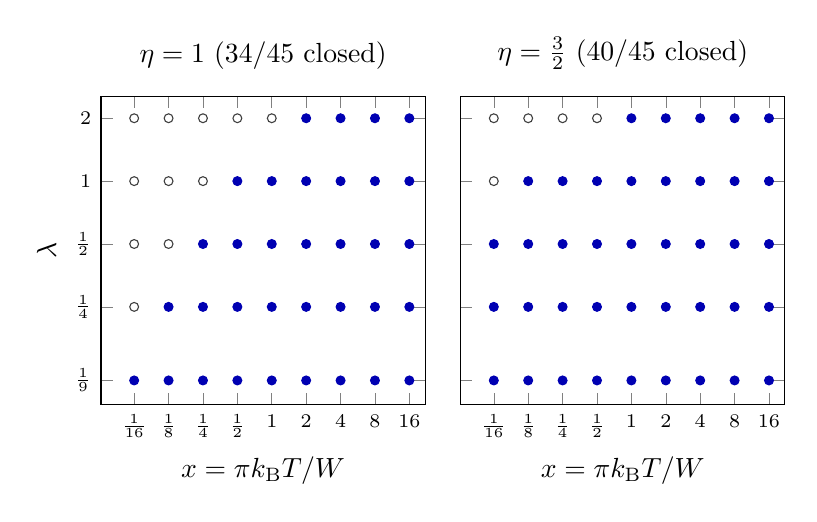
\begin{tikzpicture}
\begin{groupplot}[
  group style={group size=2 by 1,horizontal sep=0.45cm,yticklabels at=edge left},
  xmode=log, ymode=log, width=0.47\linewidth, height=5.5cm,
  xmin=0.032, xmax=22, ymin=0.085, ymax=2.55,
  xtick={0.0625,0.125,0.25,0.5,1,2,4,8,16},
  xticklabels={$\frac1{16}$,$\frac18$,$\frac14$,$\frac12$,$1$,$2$,$4$,$8$,$16$},
  ytick={0.11111111,0.25,0.5,1,2},
  yticklabels={$\frac19$,$\frac14$,$\frac12$,$1$,$2$},
  ticklabel style={font=\scriptsize}, minor tick num=0, xlabel={$x=\pi\kB T/W$},
  closed node/.style={only marks,mark=*,mark size=1.6pt,blue!70!black},
  open node/.style={only marks,mark=o,mark size=1.6pt,black!75}]
\nextgroupplot[title={$\eta=1$ ($34/45$ closed)},ylabel={$\lambda$}]
\Vfourwindows
\addplot[closed node] coordinates {
 (0.0625,0.11111111)(0.125,0.11111111)(0.25,0.11111111)(0.5,0.11111111)(1,0.11111111)(2,0.11111111)(4,0.11111111)(8,0.11111111)(16,0.11111111)
 (0.125,0.25)(0.25,0.25)(0.5,0.25)(1,0.25)(2,0.25)(4,0.25)(8,0.25)(16,0.25)
 (0.25,0.5)(0.5,0.5)(1,0.5)(2,0.5)(4,0.5)(8,0.5)(16,0.5)
 (0.5,1)(1,1)(2,1)(4,1)(8,1)(16,1)
 (2,2)(4,2)(8,2)(16,2)};
\addplot[open node] coordinates {
 (0.0625,0.25) (0.0625,0.5)(0.125,0.5) (0.0625,1)(0.125,1)(0.25,1)
 (0.0625,2)(0.125,2)(0.25,2)(0.5,2)(1,2)};
\nextgroupplot[title={$\eta=\tfrac32$ ($40/45$ closed)}]
\Vfourwindows
\addplot[closed node] coordinates {
 (0.0625,0.11111111)(0.125,0.11111111)(0.25,0.11111111)(0.5,0.11111111)(1,0.11111111)(2,0.11111111)(4,0.11111111)(8,0.11111111)(16,0.11111111)
 (0.0625,0.25)(0.125,0.25)(0.25,0.25)(0.5,0.25)(1,0.25)(2,0.25)(4,0.25)(8,0.25)(16,0.25)
 (0.0625,0.5)(0.125,0.5)(0.25,0.5)(0.5,0.5)(1,0.5)(2,0.5)(4,0.5)(8,0.5)(16,0.5)
 (0.125,1)(0.25,1)(0.5,1)(1,1)(2,1)(4,1)(8,1)(16,1)
 (1,2)(2,2)(4,2)(8,2)(16,2)};
\addplot[open node] coordinates {(0.0625,1)(0.0625,2)(0.125,2)(0.25,2)(0.5,2)};
\end{groupplot}
\end{tikzpicture}
\caption{Filled circles are \CERT\ stability nodes and open circles are unclosed nodes, not instabilities. Only the two full-coupling \PROVED\ windows are marked: shading for $x\ge19/2$ and arrows for the off-scale window $x\le2^{-40}$. The peak-box extensions to larger $x,\eta$ and smaller $\lambda$ are omitted. Unclosed regions remain.}\label{fig:coverage}
\end{figure}

%--------------------------------------------------------------------
\section{Nested flat sheets: a crossed limit that does not vanish}\label{sec:flat}

The negative half of the dichotomy uses a band in which every hypothesis of the ceiling problem except the geometry is intact. The density of states is flat, the transfer is momentum independent, the chemical potential is fixed, and the interaction is weak in the sense that $\lambda\Omega/W\to0$. In the adiabatic limit the crossed skeleton still keeps a size of order one, and the linearized pairing operator built from it lies above the ceiling.

\subsection{The bands}

\begin{definition}[Flat-sheet bands]\label{def:flat}
On $\mathcal B_1=[-\pi,\pi)$ with the normalized measure $\dd k/(2\pi)$ let
\begin{equation}\label{eq:flatdisp}
\xi(k)=W\Big(\frac{2|k|}{\pi}-1\Big)-\mu_0,\qquad |\mu_0|<W,\qquad N_0=\frac{1}{2W},\qquad A=1,
\end{equation}
with the Einstein transfer $V_j=K_j/N_0$, $K_j=\lambda\Omega^2/(\Omega^2+(2\nu j)^2)$, $M=\lambda\Omega^2$ and $\kB\Tceil=\Cinf\sqrt\lambda\,\Omega$. The band has two Fermi points $\pm k_F$ with $k_F=\frac{\pi}{2}(1+\mu_0/W)\in(0,\pi)$. Take also the two-dimensional band $\xi(k_x,k_y)=W(2|k_x|/\pi-1)-\mu_0$ on $[-\pi,\pi)^2$ with the normalized measure; it has the same density of states $A=1$, its transfer is constant, and its normal and pairing equations at fixed $k_y$ are the one-dimensional equations, so every statement below holds for it without change.
\end{definition}

Both bands are perfectly nested: the vector $2k_F$ connects the two sheets of the line, and the two-dimensional band consists of parallel flat sheets nested along $k_x$ for every $k_y$.

\subsection{The limit at fixed ratio \texorpdfstring{$\eta=T/\Tceil$}{eta}}

\begin{theorem}[Flat-sheet scaling limit]\label{thm:flat}\hfill\PROVED\\
Fix $\lambda>0$ and $\eta>0$; put $\tau=\eta\,\kB\Tceil$, $\nu=\pi\tau$, $m=\Omega/W$ and $x=\nu/W$. Then $\tau/\Omega=\eta\Cinf\sqrt\lambda$ and the Matsubara ratio $\Omega/(2\nu)=(2\pi\eta\Cinf\sqrt\lambda)^{-1}$ do not depend on $m$. Write $y=\xi/\nu$ on each sheet, that is $k=\pm(k_F+\frac{\pi\nu}{2W}y)$, and $\tilde z(n,y)=\nu z_n(\nu y)=(iw_n-y-\tilde\Sigma(n,y))^{-1}$ with $w_n=2n+1$ and $\tilde\Sigma=\Sigma/\nu$. Assume $4k_F\notin2\pi\mathbb Z$, so that $-3k_F$ is not congruent to $\pm k_F$ modulo $2\pi$; $\mu_0=-0.4W$ gives $k_F=0.3\pi$ and $-3k_F=-0.9\pi$. Then, as $m\to0$ with $\eta$ fixed:
\begin{enumerate}
\item[(i)] \emph{Sheet decomposition.} Of the eight combinations $(\sigma_k,\sigma_a,\sigma_c)\in\{\pm\}^3$, three keep the middle line in the collar: for $\sigma_k=+$ they give $\xi_b/\nu$ equal to $y_a+y_c-y$, $y_c-y_a+y$ and $y_a-y_c+y$, all of order one. In the fourth, $k_b=-3k_F+O(m)$ stays at distance $\Theta(1)$ from both Fermi points, so $|\xi_b|=\Theta(W)$, $\nu z_b=O(m)$, and that channel drops out.
\item[(ii)] \emph{The prefactors do not carry $m$.} Each sheet has weight $\frac12N_0\nu$ in $\dd k/(2\pi)=\frac12N_0\dd\xi$, so $\frac{\tau K_j}{\nu N_0}\frac{N_0\nu}{2}=\frac{K_j}{2\pi}$ and $\frac{\tau^2K_jK_l}{\nu N_0^2}\big(\frac{N_0\nu}{2}\big)^2=\frac{K_jK_l}{4\pi^2}$. The rainbow and crossed prefactors of the rescaled equations are independent of $m$.
\item[(iii)] \emph{The real rainbow shift is a translation.} On the finite band $\operatorname{Re}\Sigma_{\mathrm{RB}}(n)=-\frac{\nu}{\pi}R\log\frac{W-\mu_0}{W+\mu_0}+O(m\nu)$ holds at every order, is of order one in units of $\nu$, and is independent of $n$ up to $O(m)$. The limiting equations depend on $y$ only through $y+\operatorname{Re}\tilde\Sigma_{\mathrm{RB}}$, so on the infinite line the shift $y\mapsto y-\operatorname{Re}\tilde\Sigma_{\mathrm{RB}}$ removes it. Nothing else of $\operatorname{Re}\Sigma$ survives: the rainbow limit is purely imaginary,
\begin{equation}\label{eq:flatrb}
\tilde\Sigma_{\mathrm{RB}}(n)=\frac1\pi\sum_{j}K_j\lim_{Y\to\infty}\int_{-Y}^{Y}\tilde z(n-j,y_a)\dd y_a ,
\end{equation}
and for the bare propagator the summand equals $-i\operatorname{sgn}(w_{n-j})$.
\item[(iv)] \emph{The crossed limit does not vanish.} Collecting the three surviving channels,
\begin{equation}\label{eq:flatx}
\begin{aligned}
\tilde\Sigma_X(n,y)=+\frac{1}{\pi^2}\sum_{j,l}K_jK_l\iint_{\mathbb R^2}\frac{\dd y_a\dd y_c}{4}\Big[&\tilde z(a,y_a)\tilde z(c,y_c)\tilde z(b,y_a+y_c-y)\\
&+2\tilde z(a,y_a)\tilde z(c,y_c)\tilde z(b,y_a-y_c+y)\Big],
\end{aligned}
\end{equation}
with $a=n-j$, $c=n-l$ and $b=n-j-l$. For the bare propagator $\tilde z_0(m,y)=(iw_m-y)^{-1}$ both integrals are the Cauchy residues of Lemma~\ref{lem:residue}. They are independent of $m$ at fixed $y\ne0$, so
\begin{equation}\label{eq:flatx0}
\tilde\Sigma_X^{(0)}(n,y)=\sum_{j,l}K_jK_l\big[I_1(a,b,c;y)+2I_{23}(a,b,c;y)\big]
\end{equation}
has a finite value at every fixed $y\ne0$, and no estimate of the form $O(m)$ for the crossed self-energy can hold at fixed $\eta$.
\end{enumerate}
\end{theorem}

\begin{lemma}[Two exact residues]\label{lem:residue}\hfill\PROVED\\
For real $y\ne0$ and odd integers $w_r=2r+1$,
\begin{align}
I_1(w_a,w_b,w_c;y)&=\iint_{\mathbb R^2}\Big[\frac{\dd y_a}{2\pi}\frac{\dd y_c}{2\pi}\Big]\frac{1}{iw_a-y_a}\,\frac{1}{iw_c-y_c}\,\frac{1}{iw_b-(y_a+y_c-y)}\notag\\
&=\frac{\mathbf 1\{\operatorname{sgn}w_a=\operatorname{sgn}w_c=-\operatorname{sgn}w_b\}}{i(w_a+w_c-w_b)-y},\label{eq:I1}\\
I_{23}(w_a,w_b,w_c;y)&=+\iint_{\mathbb R^2}\Big[\frac{\dd y_a}{2\pi}\frac{\dd y_c}{2\pi}\Big]\frac{1}{iw_a-y_a}\,\frac{1}{iw_c-y_c}\,\frac{1}{iw_b-(y_a-y_c+y)}\notag\\
&=-\frac{\mathbf 1\{\operatorname{sgn}w_a=-\operatorname{sgn}w_c=-\operatorname{sgn}w_b\}}{i(w_a-w_c-w_b)+y}.\label{eq:I23}
\end{align}
The first integral is evaluated by closing the $y_c$ contour in the half plane where the summand decays: the pole at $y_c=iw_c$ contributes when $\operatorname{sgn}w_c=-\operatorname{sgn}w_b$, and the remaining $y_a$ integral picks the pole at $y_a=iw_a$ (equivalently, closing in the opposite half plane at $y_a=i(w_b-w_c)+y$) when $\operatorname{sgn}w_a=-\operatorname{sgn}w_b$ as well. The second follows from the first after $y_c\mapsto-y_c$. Because $b=n-j-l$ gives $w_a+w_c-w_b=w_n$, the first residue is the indicator of its sign condition times $\tilde z_0(n,y)$, and both residues are independent of $m$ for every fixed $y$.
\end{lemma}

Equation~\eqref{eq:flatx0} is the analytic content behind the counterexample. A crossed correction that vanished with $m$ would need these residues to cancel across the frequency sum, and that is a property of the kernel at fixed $\eta$, not a consequence of the hypotheses; the crossing below shows that no such cancellation occurs at the couplings tested.

\subsection{The crossing}

The operator of the limit is discretized on the rescaled energy line, truncated to $|y|\le Y_{\max}$ with $N_y$ points, and given $N_w$ positive Matsubara frequencies. The truncated form is not symmetric in the naive trapezoidal weighting, so the discretization is fixed once: the grid is uniform in $y$ on $[-Y_{\max},Y_{\max}]$ with spacing $\Delta y=2Y_{\max}/(N_y-1)$, interior weights $\sqrt{\Delta y}$ on each side in the $L^2(|z|^2\dd y)$ inner product, and one lumped analytical tail degree of freedom per Matsubara frequency with weight $\sqrt{\tau_n}$, projected symmetrically onto the even subspace $\mathcal H_{\mathrm{even}}$. The symmetry defect is at most $2.5\times10^{-17}$ in every run reported here.

\begin{proposition}[Crossing on the flat-sheet limit]\label{prop:flatcross}\hfill\NUM\\
Monotone continuation in $\lambda$ at $\eta=1$ gives the following top eigenvalues of the linearized pairing operator of the limit, at two discretizations and after Richardson extrapolation, together with the critical ratio $\eta_{\rm crit}$ computed at $(16,180,361)$.
\begin{center}
\begin{tabular}{lccc}
$\lambda$ & $(16,240,481)$ & $(24,180,361)$ & Richardson \\
\hline
4 & 1.003971 & 1.003043 & 1.004245 \\
6 & 1.014061 & 1.013527 & 1.013678 \\
8 & 1.015859 & 1.015679 & 1.014628 \\
\end{tabular}
\qquad
\begin{tabular}{lcc}
$\lambda$ & $\eta_{\rm crit}$ & excess over $\Tceil$ \\
\hline
4 & 1.008871 & $+0.89\%$ \\
6 & 1.045617 & $+4.56\%$ \\
8 & 1.065128 & $+6.51\%$ \\
\end{tabular}
\end{center}
Here $(N_w,Y_{\max},N_y)$ names the discretization and $\eta_{\rm crit}$ is the ratio at which the top eigenvalue reaches unity, so the linear onset sits above the ceiling by the stated excess. The Migdal--Eliashberg part of the same discretization stays below unity throughout: at $(24,180)$ its top eigenvalue is $0.968965$, $0.984313$ and $0.990572$ for $\lambda=4,6,8$. The crossing is therefore produced by the crossed skeleton and not by a failure of the rainbow equation. Each continuation used seven discretizations in $N_w$, $Y_{\max}$, $N_y$ and the spacing, and the Richardson extrapolation is first order in $1/Y_{\max}$ and second order in $\Delta y^2$ and $1/N_w^2$.
\end{proposition}

\begin{proposition}[Finite-sheet lower bounds]\label{prop:flatcert}\hfill\CERT\ (padded binary64)\\
On the periodic band of Definition~\ref{def:flat} at $\mu_0=-0.4W$, $\eta=1$ ($T=\Tceil$), and finite $m$, the largest eigenvalue of the symmetrized linearized pairing matrix of the computed normal solution satisfies
\begin{equation}\label{eq:flatcert}
\lambda_{\max}\big(K_{\rm sym}[\Sigma_{\rm num}]\big)\ge1.0090706553\qquad(\lambda=6,\ m=0.008,\ N_k=2050,\ N_w=12),
\end{equation}
\begin{equation}\label{eq:flatcert2}
\lambda_{\max}\big(K_{\rm sym}[\Sigma_{\rm num}]\big)\ge1.0123025473\qquad(\lambda=8,\ m=0.005,\ N_k=3074,\ N_w=12).
\end{equation}
\end{proposition}

The lower bounds are Rayleigh quotients formed in fifty-digit directed rounding and returned as binary64 with a padded forward-error bound, so they certify that the discretized operator at those two parameter points exceeds unity. They are not a directed-rounding enclosure of the continuum operator; their scope is the fixed discretization and the fixed numerical solution $\Sigma_{\rm num}$ at each point. At $\eta=1$ the certified Rayleigh margins above unity are $9.07\times10^{-3}$ at $(\lambda,m)=(6,0.008)$ and $1.23\times10^{-2}$ at $(\lambda,m)=(8,0.005)$, and the certificate is evaluated only at these two parameter points.

Three gaps separate Proposition~\ref{prop:flatcert} from a certification of the crossing, and each is stated with its measured size. First, the fixed-point defect. The phase-blind supremum norm of the Jacobian of the crossed map at $\lambda=6$ and $8$ is about $2.96$, above one, so a contracted remainder bound in the supremum norm does not close, and the alternative is an explicit inversion of $I-DF$ in dimension of order $10^5$. Second, the Matsubara tail. At $N_w=12$ the phase-blind rainbow tail bound on the retained window is about $0.027$, above the $0.012$ margin by which $\lambda=8$ exceeds one, while the signed shift from $N_w=12$ to $N_w=24$ is below $10^{-3}$. Third, the two limits that remove the discretization, $N_k\to\infty$ and $m\to0$. Each of the three is a quantitative task rather than a conceptual one, and none is carried out here for the band and the parameter points of this proposition. The first gap is closed in the next subsection for a smaller truncation, at $N_k=24$, $N_w=12$ and $m=1/100$ or $1/200$, where the branch is proved unique and the gap therefore no longer exists; the tail and the two limits stay open there as well.

\subsection{A certified crossing at two discretisation points}\label{sec:certified}

Proposition~\ref{prop:flatcert} certifies a Rayleigh quotient of the matrix built from a computed normal solution, and it says nothing about whether that solution is a fixed point of the truncated map. The statements below close that defect for a smaller truncation, in ball arithmetic, with a second checker and with broken variants that must be refused. They are statements about the finite model and about nothing else.

\begin{definition}[Finite two-flat-sheet model]\label{def:cert}
Let $W=1$. The momenta and the dispersion are
\begin{equation}\label{eq:certgrid}
k_j=-\pi+\Big(j+\tfrac12\Big)\frac{2\pi}{N_k},\qquad \xi_j=2\,\frac{|2j+1-N_k|}{N_k}-1-\mu_0,\qquad j=0,\dots,N_k-1,
\end{equation}
so the two branches have equal length and the combined density of states is $A=1$, $N_0=\tfrac12$. The Matsubara frequencies are $\omega_n=2n+1$ for $n=-N_w,\dots,N_w-1$, hence $M=2N_w$ of them. The temperature is fixed at the ratio $\eta$ of the ceiling, $\tau=\eta\Cinf\sqrt\lambda\,m$, and $\nu=\pi\tau$. The Einstein kernel is $K(d)=m^2/(m^2+(2\pi\tau d)^2)$, the rainbow and crossed couplings are
\begin{equation}\label{eq:certcouple}
g_{\rm RB}=2\lambda\tau,\qquad C_X=\Big(\frac{2\lambda\tau}{N_k}\Big)^2,
\end{equation}
evaluated inside the enclosure from exact rational parameters and the decimal constant $\Cinf=0.18272624777232952$, and the propagator is $z(n,j)=\big(i\omega_n\nu-\xi_j-\Sigma(n,j)\big)^{-1}$. With all momenta read modulo $N_k$, the normal-state map is
\begin{equation}\label{eq:certphi}
\begin{aligned}
\Phi(\Sigma)(n,j)={}&g_{\rm RB}\sum_a K(n-a)\,\frac{1}{N_k}\sum_m z(a,m)\\
&+C_X\!\!\sum_{\substack{a,c\\0\le a+c-n<M}}\!\!K(n-a)K(n-c)\sum_{m,m'}z(a,m)\,z(c,m')\,z\big(a+c-n,\,m+m'-j\big),
\end{aligned}
\end{equation}
and terms with $a+c-n\notin[0,M)$ are omitted, which is part of the definition of the truncated model. Write $\mathrm{az}(n,j)=|z(n,j)|$, $u=(j_0-j)\bmod N_k$, $b'=p+a_0-n$ and $w=(j_0+j)\bmod N_k$. The linearised gap operator, with $c=a_0-a+n$ in its last sum, is
\begin{equation}\label{eq:certB}
\begin{aligned}
B(\Sigma)_{(n,j),(a_0,j_0)}=\mathrm{az}(n,j)\,\mathrm{Re}\Big\{&\mathrm{az}(a_0,j_0)\Big[\frac{g_{\rm RB}K(n-a_0)}{N_k}\\
&\quad+2C_XK(n-a_0)\!\!\sum_{\substack{p\\0\le b'<M}}\!\!K(n-p)\sum_m z(p,m)z(b',m+u)\Big]\\
&+C_X\,\mathrm{az}(a_0,j_0)\!\!\sum_{\substack{a\\0\le c<M}}\!\!K(n-a)K(n-c)\sum_m z(a,m)\overline{z(c,w-m)}\Big\}.
\end{aligned}
\end{equation}
Every constant in \eqref{eq:certgrid} to \eqref{eq:certB} is computed inside the enclosure from exact integers and rationals and is never lifted from a rounded float. The map is not projected onto inversion-even self-energies, so the top eigenvalue below is that of the unprojected operator. These are the formulas of the discrete solver used for Proposition~\ref{prop:flatcert}, transcribed term for term; the certificate and the second checker were written against this statement rather than against that solver's code, and their agreement with its output is a check on the transcription.
\end{definition}

\begin{proposition}[The gap operator is real symmetric]\label{prop:sym}
For every $\Sigma\in\mathbb C^{M\times N_k}$, with no symmetry assumed on $\Sigma$, the matrix \eqref{eq:certB} satisfies $B(\Sigma)=B(\Sigma)^{\mathsf T}$.
\end{proposition}

\begin{proof}
Write $B_{(n,j),(a_0,j_0)}=\mathrm{az}(n,j)\,\mathrm{az}(a_0,j_0)\,\mathrm{Re}(T_1+T_2+T_3)$, where $T_1$, $T_2$, $T_3$ are the three inner terms of \eqref{eq:certB}. The amplitudes $\mathrm{az}$ are real and the prefactor is symmetric, so it suffices to transpose the inner terms.

$T_1=g_{\rm RB}K(n-a_0)/N_k$: the kernel is even, $K(-d)=K(d)$, because it is a function of $d^2$.

$T_2=2C_XK(n-a_0)\sum_{p}K(n-p)\sum_m z(p,m)z(p+a_0-n,\,m+u)$ with the constraint $0\le p+a_0-n<M$. In the transposed entry the kernel factor is $K(a_0-n)=K(n-a_0)$, the shift is $u'=-u\bmod N_k$, and the constrained index is $s=p+n-a_0\in[0,M)$. Writing the transposed summand with that letter, $K(n-s)\,z(s+a_0-n,\,m)\,z(s,\,m-u)$, and relabelling $m\mapsto m+u$ (the second index of $z$ is a momentum index taken modulo $N_k$, so the shift relabels the $N_k$ terms) gives $K(n-s)\,z(s+a_0-n,\,m+u)\,z(s,m)$: the original summand with $p=s$. Hence $T_2$ is symmetric.

$T_3=C_X\sum_{a}K(n-a)K(n-c)\sum_m z(a,m)\overline{z(c,w-m)}$, where $c=a_0+n-a$ is the constrained index $0\le c<M$ and $w=(j_0+j)\bmod N_k$. In the transposed entry the constrained index is again $c=a_0+n-a$, and $w$ is unchanged because it is symmetric in $(j,j_0)$. From $a+c=a_0+n$ we have $a_0-a=c-n$ and $a_0-c=a-n$, so the transposed weights $K(a_0-a)K(a_0-c)$ equal $K(n-c)K(n-a)$ by evenness of $K$, and the inner sum is the same sum term by term. Hence $T_3$ is symmetric.

Taking real parts, each entry of $B$ equals the corresponding entry of $B^{\mathsf T}$.
\end{proof}

Numerically, the symmetry is not an artefact of inversion-even data: at $N_k=8$ and $N_k=10$ with random non-inversion-even perturbations of relative size $10^{-3}$ in the supremum norm, the largest entry of $B-B^{\mathsf T}$ is $5.55\cdot10^{-17}$ against an operator norm of order one. That check is \NUM, as a check must be; the symmetry itself is the proposition.

\begin{theorem}[Fixed point and crossing on a ball, certified]\label{thm:C}\hfill\CERT\\
Let $\mathcal M(24,12;\lambda,m,\eta,\mu_0)$ be the model of Definition~\ref{def:cert} with $N_k=24$ momenta, $N_w=12$ ($M=24$, $D=MN_k=576$ unknowns), $\lambda=8$, $\eta=1$, $\mu_0=-2/5$ and $m\in\{1/100,1/200\}$, and let $\Sigma_0\in\mathbb C^{M\times N_k}$ be the normal-state fixed-point candidate of record R7 at that point, lifted exactly into the ball type. Fix $\rho=10^{-12}$ and $\theta=5\cdot10^{-3}$, and let $\mathrm{Box}(\Sigma_0,\rho)$ be the closed complex box in which every real and imaginary component of $\Sigma-\Sigma_0$ is bounded by $\rho$; it contains the sup-norm ball of radius $\rho$. Then:
\begin{enumerate}
\item[(N)] \emph{Fixed point.} $\Phi$ has exactly one fixed point $\Sigma^\star$ in the sup-norm ball of radius $\rho$, and
\begin{equation}\label{eq:certN}
\|\Sigma^\star-\Sigma_0\|_\infty\le\frac{r}{1-k}\le\begin{cases}5.83329104641\cdot10^{-17}, & m=1/100,\\ 3.63702630192\cdot10^{-17}, & m=1/200,\end{cases}
\end{equation}
with $r\le5.83329104451\cdot10^{-17}$, $k\le3.25923499198\cdot10^{-10}$ at $m=1/100$ and $r\le3.63702630028\cdot10^{-17}$, $k\le4.50507433578\cdot10^{-10}$ at $m=1/200$. Here $A=\big(I-D\Phi(\Sigma_0)\big)^{-1}$ is lifted exactly, $r=\|A(\Phi(\Sigma_0)-\Sigma_0)\|_\infty$ and $k=\|I-A\big(I-D\Phi(\mathrm{Box})\big)\|_\infty$, where $D\Phi$ is enclosed over the whole box; the containment $r+k\rho\le\rho$ and $k<1$ hold for both parameter sets. No contraction of $\Phi$ itself is used or asserted.
\item[(K)] \emph{Crossing on the whole box.} For every $\Sigma\in\mathrm{Box}(\Sigma_0,\rho)$,
\begin{equation}\label{eq:certK}
\lambda_{\max}\big(B(\Sigma)\big)\ge1+\theta,\qquad
\lambda_{\max}\big(B(\Sigma)\big)\ge\begin{cases}1.00579751250,&m=1/100,\\1.01993371122,&m=1/200,\end{cases}
\end{equation}
so the Rayleigh bound clears the threshold $1+\theta$ by at least $7.97512500371\cdot10^{-4}$ at $m=1/100$ and $1.49337112263\cdot10^{-2}$ at $m=1/200$, and therefore exceeds unity itself by at least $5.7975125\cdot10^{-3}$ and $1.993371122\cdot10^{-2}$. The bound is the symmetric Rayleigh quotient $\langle v,Bv\rangle/\langle v,v\rangle$ for a fixed real vector $v$, evaluated in ball arithmetic and decided on its lower endpoint; Proposition~\ref{prop:sym} makes it a bound on $\lambda_{\max}(B)$ itself, with no antisymmetry penalty. In particular $\lambda_{\max}\big(B(\Sigma^\star)\big)>1$ at the fixed point of (N).
\item[(S)] \emph{Second checker.} A separately written checker, with its own transcription of \eqref{eq:certphi} to \eqref{eq:certB}, its own directed-rounding interval arithmetic at 160 bits and its own box construction, reproduces both inequalities of (N) for both parameter sets, with $r\le1.43466873225\cdot10^{-16}$, $k\le1.53363171691\cdot10^{-9}$ at $m=1/100$ and $r\le1.00667718670\cdot10^{-16}$, $k\le2.06306136514\cdot10^{-9}$ at $m=1/200$. It reproduces (K) at the coarser momentum grid $N_k=8$, $m=1/100$, where $\lambda_{\max}\ge1.03881800695$, and at $N_k=24$, $m=1/100$, where $\lambda_{\max}\ge1.00579751243$. At $N_k=24$, $m=1/200$ it also reproduces (K), with $\lambda_{\max}\ge1.01993371112$. The ten broken variants and the 400-bit reproduction described below belong to the same record and guard the same decisions.
\item[(V)] \emph{Vertex-decisiveness, \NUM\ and not certified.} On the same lattices the rainbow-only column gives $\lambda_{\rm ME}=0.980079149$ at $m=1/100$ and $\lambda_{\rm ME}=0.994520242$ at $m=1/200$ in binary64, so the rainbow kernel alone stays below unity at the ceiling; no certified upper bound on $\lambda_{\rm ME}$ is computed.
\end{enumerate}
\end{theorem}

\paragraph{How the certificate is decided.} The enclosure is built from the box of Definition~\ref{def:cert} as the hull of the two endpoints $\Sigma_0\pm\rho$ componentwise, and a guard rejects any enclosure whose radii fall below $\rho/2$, so that a rounding-size ball can no longer be passed off as the box. A second guard rejects an enclosure in which a certified coupling has radius zero, which would mean that a rounded binary64 value had been lifted as if exact. Every printed number is a guaranteed decimal read from the lower or the upper endpoint of the corresponding ball, never from a midpoint, and the pass or fail of a comparison is decided on endpoints with no strict inequality against a ball. At $m=1/100$ the distance from the box to the nearest propagator pole is at least $0.0565776818037$ and at $m=1/200$ at least $0.0384152648904$, so $\Phi$ and $D\Phi$ are holomorphic on the box and the mean-value estimate underlying the radii test applies. This guards precisely the defects that an earlier version of the record carried, where the box was not a box, a binary64 $1/N_k$ and a rounded $1.2$ entered the enclosures, balls were compared with strict inequalities in the reductions, and a perturbation inequality for nonsymmetric matrices, false in general, stood in for the symmetry argument.

\paragraph{Higher precision and refused variants.} Doubling the working precision from 200 to 400 bits reproduces both bounds and both radius pairs to every printed digit, with exit code zero. Ten deliberately broken variants are refused, each with the pass criterion its fault attacks, and each with nonzero exit:
\begin{center}
\small
\begin{tabular}{@{}>{\raggedright\arraybackslash}p{4.6cm}ll@{}}
\hline
fault & surviving quantity & reading \\
\hline
crossed term removed from the model & $\lambda_{\max}\ge0.9800791489$ & below unity \\
model moved to $m=2/100$ & $\lambda_{\max}\ge0.9969667560$ & below unity \\
zero-radius box ($\rho=0$) & $r\le5.834\cdot10^{-17}$ (not $\le0$) & containment fails \\
residual inflated by $2^{20}$ & $r\le6.117\cdot10^{-11}$ (not $\le\rho$) & containment fails \\
rainbow prefactor $6/5$, map a further $6/5$ & $r\le8.946\cdot10^{-2}>\rho$ & containment fails \\
threshold raised to $1.01$ & $1.00579751250<1.01$ & margin fails \\
diagonal lowered by $2\cdot10^{-2}$ & $\lambda_{\max}\ge0.9857975125$ & below unity \\
third term of \eqref{eq:certB} dropped & $\lambda_{\max}\ge0.6967262045$ & below unity \\
a point certified instead of a box & box guard & enclosure refused \\
couplings lifted from binary64 & constant guard & enclosure refused \\
\hline
\end{tabular}
\end{center}
Each entry is the guaranteed bound or the failure value printed by the corresponding run.

\paragraph{Adjacent discretisations, \NUM.} The same diagnostics report top eigenvalues of $1.0074033857$ at $N_k=48$, $1.0073349348$ at $N_k=64$, $1.0054800598$ at $N_w=16$ and $1.0061798062$ at $\lambda=6$ with the certified $N_k$, $N_w$ and $m=1/100$, and $0.9969667561$ at $m=2/100$, which lies below the crossing. At $m=1/400$ the value is $1.0681283523$, but the rainbow column alone already crosses there, at $1.0254$, so that point does not isolate the vertex effect. These numbers are binary64 eigenvalues printed as diagnostics, not enclosures; they indicate that the certified point is not an isolated feature of the momentum grid in the directions tested, and they do not substitute for the tail and continuum bounds that remain open.

\paragraph{What the theorem does not say.} Theorem~\ref{thm:C} is a certified statement about the finite discretised model of Definition~\ref{def:cert}. It is not a statement about the continuum operator, it carries no bound on the Matsubara tail, it is not a measured $T_c$ and not a material, and it does not address the charge and Peierls instabilities of the nested band discussed next. Its role is to remove the first of the three gaps from the certification problem, at two discretisation points, so that the remaining requirement is quantitative in $N_w$, $N_k$ and $m$.

\begin{remark}[Charge response and the status of the branch]\label{rem:cdw}
The band of Definition~\ref{def:flat} is nested, and its static charge response at the nesting vector is large: the product of the resummed interaction with the static susceptibility at $2k_F$ runs from $8.41$ to $10.37$ over $\lambda=6,8$ and $m=0.005$ to $0.012$. A value above one means that the random-phase resummation of the same interaction is unstable at $2k_F$, so a charge or Peierls instability competes with, and in the mean-field sense precedes, the pairing instability of the truncated equations. The normal branch is therefore not the physical ground state of that band, and this section is a statement about the equations and their ceiling, not about a material. What it does establish is the logical point: bounded $A$, constant $V_j$ and fixed $\mu$ do not imply the ceiling.
\end{remark}

The failure is not caused by an unbounded density of states, by a momentum-dependent coupling, or by a chemical potential that moves with the phonon scale. What the flat sheets lose is the curvature that made the three energy slabs of the small-$x$ estimate intersect in a set of vanishing measure; on a nested band the middle line sits on the Fermi surface along a whole one-parameter family of the two momenta, and the excess survives the limit. That contrast is the content of Section~\ref{sec:curved}.

%--------------------------------------------------------------------
\section{Curved Fermi surfaces: a universal small-\texorpdfstring{$x$}{x} window}\label{sec:curved}

The positive half replaces the spherical joint density by a coarea estimate and a layer-cake reduction. Neither step uses rotational symmetry: the sphere enters only through the constancy of its curvature and through the explicit value of its admissibility constant. The hypotheses constrain the dispersion and the normal branch, and the conclusion is a statement about the relative size of the crossed form in the adiabatic window.

\begin{definition}[Curvature class]\label{def:curved}
Let $d\ge2$, let $\xi\in C^2(\mathcal B)$ on a compact band domain $\mathcal B\subset\mathbb R^d$ be inversion-even, $\xi(-\mathbf k)=\xi(\mathbf k)\in[-W,W]$, and let $\nu=\pi\tau$. Assume
\begin{enumerate}
\item[(H1)] on the collar $\{|\xi|\le\varepsilon_0\}$ the gradient does not vanish, $|\nabla\xi|\ge v_{\min}>0$, and $|D^2\xi|\le M_2$;
\item[(H2)] the density of states is normalized by $0<N_0=N(0)<\infty$ and bounded by $N(\xi)\le AN_0<\infty$, and the transfer obeys $0\le V_j(\mathbf q)=V_j(-\mathbf q)=V_{-j}(\mathbf q)\le\vmax K_j/N_0$;
\item[(H3)] every level set $\Sigma_\xi$ in the collar is a finite union of smooth strictly convex $C^2$ hypersurfaces with all principal curvatures at least $\kappa_{\min}>0$, and for distinct components with parallel or antiparallel normals the relative curvature is nondegenerate, $\det(\Pi_b\mp\Pi_c)\ne0$ at every critical pair $(\mathbf k_b^*,\mathbf k_c^*)$.
\end{enumerate}
\end{definition}

Hypothesis (H3) says that the neighbouring energy surfaces of the collar are strictly convex, that their principal curvatures stay bounded below by $\kappa_{\min}>0$, and that any parallel or antiparallel tangency between distinct components has nondegenerate relative curvature $\det(\Pi_b\mp\Pi_c)\ne0$. The geometric constant $\Cgeom$ depends only on $v_{\min}$, $M_2$, $\kappa_{\min}$, $\varepsilon_0$ and the number of components.

\begin{lemma}[Coarea curvature suffices for the strip overlap]\label{lem:coarea}\hfill\PROVED\\
Let $\xi$ satisfy the hypotheses of Definition~\ref{def:curved}. For $I_k(u_a,u_b,u_c)$ the normalized integral of $\mathbf 1\{|\xi_a|\le u_a\}\mathbf 1\{|\xi_b|\le u_b\}\mathbf 1\{|\xi_c|\le u_c\}$,
\begin{equation}\label{eq:coarea}
I_k(u_a,u_b,u_c)\le \Cgeom (AN_0)^2\,\frac{u_au_bu_c}{W^{\alpha}}\min(u_a,u_b,u_c)^{\alpha-1}\Big(1+\log_+\frac{W}{\min(u_a,u_b,u_c)}\Big)^{\beta},
\end{equation}
with $\alpha=1$, $\beta=1$ in $d=2$ and $\alpha=1$, $\beta=0$ in $d\ge3$, and a constant $\Cgeom$ that depends on $v_{\min}$, $M_2$, $\kappa_{\min}$, $\varepsilon_0$ and the number of components only.
\end{lemma}

The proof is invariant under permutations of $(u_a,u_b,u_c)$, so the smallest slab can be called $u_1$. A slab thicker than the collar is bounded by dropping its indicator and using the density-of-states bound twice. Inside the collar the coarea formula on the two remaining momenta turns each slab into a thickness divided by $|\nabla\xi|$, and the inner integral of the middle slab is bounded by its width divided by the modulus of the tangential gradient. That modulus is bounded below off the tangency sets, where the two level sets cross transversally. Near a forward tangency the Gauss map of a strictly convex level set is bilipschitz with constant $1/\kappa_{\min}$, so the configuration collapses to a ball around the point, and the remaining collar is controlled by the second variation of $\xi$ along the tangential direction. Near an antiparallel tangency the quadratic expansion in $2(d-1)$ tangential variables is positive definite with a lower bound proportional to $v_{\min}\kappa_{\min}$, so its slab has measure of order $u_2$. The logarithmic factor of $d=2$ comes from the annular integral over the distance between the two lower-dimensional level sets; in $d\ge3$ that integral converges at the lower end and the logarithm is absent.

Two features of Lemma~\ref{lem:coarea} matter for the dichotomy. The bound is uniform in the shapes of the level sets once their curvatures are bounded away from zero, which is what turns a spherical statement into a geometric one. And the same estimate fails on the nested band of Section~\ref{sec:flat}, where two of the three slabs are parallel and their intersection is a segment of fixed length; in $d=1$ there is no tangential direction at all. The convexity hypothesis therefore cannot be replaced by nesting or by small curvature.

\begin{lemma}[Layer-cake reduction]\label{lem:layercake}\hfill\PROVED\ with \CERT\ constants\\
Assume (H1) to (H3) and write $D_n(\xi)=(\omega_n^2+\xi^2)^{-1/2}$ and $x=\nu/W\le1$. Then for every $\mathbf k$ and all Matsubara indices $a,b,c$,
\begin{equation}\label{eq:layercake}
\mathcal J_3(\mathbf k;a,b,c)=\iint_{\mathcal B^2}D_a(\xi_a)D_b(\xi_b)D_c(\xi_c)\dd\mu(\mathbf k_a)\dd\mu(\mathbf k_c)\le\frac{\CLC}{\nu}(AN_0)^2x^{\alpha}\Big(1+\log_+\frac1x\Big)^{3+\beta},
\end{equation}
uniformly for $\alpha\in(0,1]$, with $\CLC=3\Cgeom+34$. The numerical constants entering $\CLC$ are certified in the replay supplement ($2\sqrt2<3$ and $24\sqrt2<34$); the same supplement certifies the Young-ball constants of Theorem~\ref{thm:curved}(1) ($c_{\mathrm H}<4$ for the triple-H\"older constant, image $<0.3187<1/3$, Lipschitz constant $<0.9340<1$, and $u_n/|\omega_n|\ge2/3$).
\end{lemma}

The reduction uses $(m^2+\xi^2)^{-1/2}\le\sqrt2\max(m,|\xi|)^{-1}=\sqrt2\int_m^\infty u^{-2}\mathbf 1\{|\xi|\le u\}\dd u$, which is an identity of the layer cake and is sharp at $|\xi|=m$, so each power of a propagator becomes one layer. Multiplying the three layers and using $|\omega_n|\ge\nu$, the region where one layer exceeds $W$ contributes $24\sqrt2\,\nu^{-1}(AN_0)^2x(1+\log_+(1/x))^2$ with the density-of-states bound $\int\mathbf 1\{|\xi|\le u\}\dd\mu\le\min(2AN_0u,1)$, and the region where all three stay below $W$ contributes $3\Cgeom\nu^{-1}(AN_0)^2x^\alpha(1+\log_+(1/x))^{3+\beta}$ by Lemma~\ref{lem:coarea} with $\min(u_a,u_b,u_c)^{\alpha-1}\le\nu^{\alpha-1}$. The sum of the two is the stated constant, with no singularity as $\alpha\to1^-$.

\begin{theorem}[Two regular regimes on curved Fermi surfaces]\label{thm:curved}\hfill\PROVED, with the scope stated in each part\\
Write $\nu=\pi\tau$, $x=\nu/W$, $B=\max(1,A\vmax R)$ and $\rho=m\sqrt\lambda$.
\begin{enumerate}
\item[(1)] \emph{All $x$: Young ball under a constant transfer and an even density of states.} Assume $V_j=K_j/N_0$, $N(-\xi)=N(\xi)$ and $\lambda\le\Lambda<\infty$. At any $\tau>0$ with $AR(\tau)\le1/9$ the regular solution is unique within $\|\Sigma\|_\infty\le\nu/3$ with $u_n|\omega_n|^{-1}\ge2/3$, and pairing has absolute Schur bound strictly below one. The criterion holds at every $\tau\ge\tau_Y$ if $A\lambda<1/9$, with
\begin{equation}\label{eq:curvedV3b}
\kB\Tlin\le\tau_Y=\frac{9\,AM_1}{2(1-9A\lambda)},\qquad M_1=\int\Omega\dd\lambda(\Omega),
\end{equation}
and if $A\lambda\le1/26^2$ then $\tau_Y\le(117/667)\sqrt{AM}<\Cinf\sqrt{AM}$, with no adiabatic assumption and no curvature hypothesis. Both extra hypotheses are needed for a statement valid at every $x$: without a particle--hole-even density of states and a constant transfer, the bare rainbow shift $\operatorname{Re}\Sigma^{(0)}_{\mathrm{RB}}=\Theta(\nu A\vmax R\log(1/x))$ leaves every ball of fixed radius as $x\to0$, however small $AR$ is.
\item[(2)] \emph{Small $x$: crossed correction in the adiabatic window.} Assume (H1) to (H3) and let a sign-preserving normal branch exist with $u_n(\mathbf k)\ge c_0|\omega_n|$, $c_0\in(0,1]$, and $|\operatorname{Re}\Sigma_n(\mathbf k)|\le\Delta_R$. Put $\gamma=1+\Delta_R/(c_0\nu)$; in the small-shift regime $\Delta_R\le c_1\nu$ one has $\gamma=O(1)$, and for $\Delta_R\le C_{\mathrm{Re}}\nu(1+\log_+(1/x))$ the factor $\gamma^3$ adds at most three logarithmic powers and preserves the vanishing in $x$. Then
\begin{equation}\label{eq:curvedLX}
L_X\le\frac{\gamma^3c_0^{\alpha-1}\CLC}{\pi^2}B^2x^{\alpha}\Big(1+\log_+\frac{1}{c_0x}\Big)^{3+\beta},\qquad |F_X[y]|\le10L_XQ_0[y],
\end{equation}
For a constant transfer $V_j=K_j/N_0$, splitting $y=\bar y+y_\perp$ into the $|Q|$-weighted mean over the momentum measure and its orthogonal part gives
\begin{equation}\label{eq:curvedF}
F[y]\ge\big(1-\sS(b)-10L_X\big)Q_0[\bar y]+\big(1-10L_X\big)Q_0[y_\perp],
\end{equation}
with $b_n=\frac{1}{\pi AN_0}\int u_n\dd\mu/(u_n^2+(\xi+\operatorname{Re}\Sigma_n)^2)\in(0,1]$. There is therefore a window $x\le x_*(B,\text{geometry})$ in which, on that same branch,
\begin{enumerate}
\item[(i)] for a constant transfer and an even density of states, whose branch lies within $O(\nu L_X)$ of the purely imaginary rainbow solution, one has $|{\sS(b)-\sS(b^*)}|=O(L_X)$ and hence $\kB\Tlin\le\Cinf\sqrt{AM}\,(1+C_3B^2\rho^{\alpha}(1+\log_+(1/\rho))^{3+\beta})$ with an explicit $C_3$, while the ME onset of the branch is shifted by a relative factor at most $1+O(L_X)$;
\item[(ii)] for a constant transfer $V_j=K_j/N_0$ and a general asymmetric density of states, where $b_n\le1$ does not imply $\sS(b)\le\sS(1)$ because $S(b)$ carries a negative normal-mass diagonal, the comparison is with $\frac{1}{\pi\sqrt2}\sqrt{AM}$ on every positive time-reversal-reflected branch, with the same relative correction $1+C_3B^2\rho^\alpha(1+\log_+(1/\rho))^{3+\beta}$, and the momentum-resolved ME onset of that branch is shifted by a relative factor at most $1+O(L_X)$;
\item[(iii)] for a general momentum-dependent transfer $0\le V_j\le\vmax K_j/N_0$, where only $F[y]\ge Q_0[y]+F_{\mathrm{ME}}[y;u]-10L_XQ_0[y]$ holds and the split of the pairing form is unavailable, the first crossed skeleton shifts the momentum-resolved ME onset of that branch by a relative factor at most $1+O\big((A\vmax R)^2\rho^{\alpha}(1+\log_+(1/\rho))^{3+\beta}\big)$.
\end{enumerate}
\end{enumerate}
\end{theorem}

Part (1) is the Young-ball closure of the earlier version, restated as the all-$x$ half of the dichotomy; its statement, its proof and its constants are unchanged, and the particle--hole symmetry and the constant transfer appear there as hypotheses rather than as conveniences. Part (2) is the exact form of the statement that the small-$x$ exclusion of the spherical model is not an artifact of the sphere. The sphere satisfies (H1) to (H3): in its collar the level sets are spheres, the gradient is bounded away from zero, and the principal curvatures equal $1/|k|$, which is bounded below on the collar. Theorem~\ref{thm:V3a} keeps its statement and its proof and is recovered from part (2) with the spherical admissibility constant.

What part (2) does not do is part of its content. The window is small $x$ at fixed $\lambda$, so it does not reach the intermediate-$x$ region where the crossed correction competes with a right-hand side that stays of order one. The comparison is against the ME onset on the same branch, and against the ceiling itself only in the symmetric case of (2)(i). And the conclusion is one-sided by construction: it shows that the crossed skeleton cannot raise the onset by more than a relative amount that vanishes with $x$, and it asserts nothing about a decrease.

%--------------------------------------------------------------------
\section{Proof sketches}\label{sec:proofs}

Full proofs are in the record files (R0 to R7) named in each paragraph, which are supplementary material to this preprint; the mapping from numbered statements to record, section and line is in the accompanying claims table. What follows records the structure only.

\subsection{The signed identity}

\begin{lemma}[Signed identity, momentum-resolved]\label{lem:signed}
Assume $V_s\ge0$ and separately even in momentum and frequency. On a sign-preserving branch put $z_p=(i\omega_p-\xi_p-\Sigma_p)^{-1}=r_p-iQ_p$, $u_p=\omega_p-\operatorname{Im}\Sigma_p$ and $Q_p=u_p|z_p|^2$, so $\omega_p Q_p>0$. Take a real even-frequency singlet trial $\varphi$ in the inversion-even momentum sector and set $y=\varphi/u$. Take minus the imaginary part of the normal equation, multiply by $y_p$, subtract the anomalous equation and test with $Q_p y_p$. Reanchoring gives $F=Q_0+F_{\Rg}+F_X$:
\begin{align}
Q_0&=\int\omega_p Q_p|y_p|^2,\qquad F_{\Rg}=\frac\tau2\int V_s Q_pQ_a|y_p-y_a|^2,\\
F_X&=\tau^2\!\int V_s V_t\Big[-\tfrac14 Q_pQ_aQ_bQ_c|y_p-y_a+y_b-y_c|^2\nonumber\\
&\hspace{8em}+\tfrac12\sum_{v=a,b,c}Q_pQ_v r_{v'}r_{v''}|y_p-y_v|^2\Big],
\end{align}
where $v$ ranges over three corner occurrences and $v',v''$ denote the other two. Polarization extends the identity to complex trials in the same parity sector.
\end{lemma}

\noindent\emph{Source.} R2 \texttt{RIGOR.md}, \S1, lines 3--29. The first term of $F_X$ is the alternating four-corner square, the second the three real-line-weighted pair squares. Keeping only the four-corner square misses a genuine forward contribution. The identity is exact; the review audited the signs, the coefficients and the form domain and found the record acceptable as a whole.

\begin{lemma}[Local reduction, four-corner square]\label{lem:local}
Under the centered flat-band normal-branch hypotheses of Theorem~\ref{thm:V1}, write $a=n-j$, $b=n-j-l$, $c=n-l$, $w_n=2n+1$, $s_n=|u_n|/(\pi\tau)$, $\sigma_n=\operatorname{sgn}(w_n)=\operatorname{sgn}(u_n)$ and $b_n=\tfrac2\pi\arctan(W/(\pi\tau s_n))$. Set $q_n=\sigma_n b_n$, $y_n=\varphi_n/u_n$, $\kappa=\pi^2\tau N_0=\pi^2\tau/(2W)$. The equations are
\begin{align}
\frac{u_n}{\pi\tau}&=w_n+\sum_jK_jq_a-\kappa\sum_{j,l}K_jK_l\,q_aq_bq_c,\nonumber\\
\frac{\varphi_n}{\pi\tau}&=\sum_jK_jq_ay_a-\kappa\sum_{j,l}K_jK_l\,q_aq_bq_c\,(y_a-y_b+y_c),\label{eq:localeq}
\end{align}
and the four-corner average is
\begin{equation}\label{eq:QX}
Q_X=-\frac\kappa4\sum_{n,j,l}K_jK_l\,q_nq_aq_bq_c\,|y_n-y_a+y_b-y_c|^2,
\end{equation}
with all terms having $j=0$ or $l=0$ vanishing. Counting coincident corners with multiplicity gives $|Q_X|\le16\kappa L^2\sum_n b_n|y_n|^2\le4X\|f\|_2^2$, where $X=4\kappa L^2$ and $f_n=\sqrt{|w_n|b_n}\,y_n$.
\end{lemma}

\noindent\emph{Source.} R1 \texttt{RIGOR.md}, \S1 (equations 3--5 of that record). The cancellation in~\eqref{eq:QX} (terms with $j=0$ or $l=0$ vanish) is the vertex-specific content of the proof. The hypotheses are exactly those of Theorem~\ref{thm:V1}, so $\chi_n=0$ and the reflected widths are positive. A nonzero real shift $\chi_n$ is excluded, and the displayed arctangent weight $b_n$ and the local reduction are not asserted for it.

Before folding, note the convention used throughout. The bound in~\eqref{eq:QX} is a ledger entry on the full signed line, where $\|f\|_2^2$ is summed over all integers $n$. On the odd subspace, reflection halves both the full-line crossed form and the squared norm, so the same normalized bound holds on the positive half-line. The folded ledger below therefore inherits the value $4X$, not $2X$.

In the folded $f$ coordinates ($n,m\ge0$), set $D_{nm}=K_{|n-m|}$, $H_{nm}=K_{n+m+1}$ and $P_{nm}=D_{nm}-H_{nm}$. The canceled ME form is $I-S(b)$ with entries
\begin{align*}
 S(b)_{nm}&=\frac{\sqrt{b_nb_m}(D_{nm}+H_{nm})}{\sqrt{w_nw_m}},\quad n\ne m,\\
 S(b)_{nn}&=\frac{2H_{nn}b_n-\sum_{m\ne n}P_{nm}b_m}{w_n}.
\end{align*}

\begin{lemma}[Scalar comparison (imported)]\label{lem:import}
$\sup\sigma S(1)\le\Cinf^2M/\tau^2$.
\end{lemma}

\noindent The scalar input \cite{RensScalar} bounds the unit-weight comparison $S(1)$, not the raw Cooper operator. In the canceled matrix $K_0$ drops out and the soft transfer envelope is $M/(2\pi\tau j)^2$ for $j\ge1$.

\subsection{Theorem~\ref{thm:V1}}

On the centered normal widths the comparison is $\sup\sigma S(b)\le\sup\sigma S(1)+D_*$, where
\[
D_*=\frac{2\tau}{W}\big[2L+K_1+(\lambda+2L+X)K_1\big].
\]
For $\tau\ge\tau_0=\Cinf\sqrt M$, put $r=\tau_0/\tau$. Then $L\le M/(24\tau^2)\le\tfrac43r^2$ and $X\le\tfrac{20}{3}\rho r^3$, giving $D_*+4X\le r\epsilon$. The form is bounded below by $(1-r^2-r\epsilon)I$, strictly positive at $\tau\ge\tau_0(1+\epsilon)$. For fixed $\lambda$ the scalar gap $\delta_\lambda$ instead pays this loss when $\epsilon<\delta_\lambda$.

Separately, on $[\tau_0,2\tau_0]$ with $(1+\lambda)\rho\le1/100$, Brouwer's theorem on finite positive-frequency boxes with bounds $w_n-7/8$ and $w_n+\lambda+2L+X$ for $n\ge0$, reflected to negative frequencies, gives pointwise existence by diagonal extraction and dominated convergence. The full proof is R1 \texttt{RIGOR.md}, \S1.

\subsection{Proposition~\ref{prop:obstruction} and Theorem~\ref{thm:V2}}

The obstruction of Proposition~\ref{prop:obstruction} is by direct integration of the three-line triangle at $\tau=\Omega$ in the limit $m\to0$ (R1 \texttt{RIGOR.md}, \S2). For Theorem~\ref{thm:V2}(i) one controls $r=B/(\pi^2\tau)$ with $B=\sum_j\!\int V_j$: positivity, monotone integral comparison and the Einstein kernel give $B/B_0\le1+\Omega/(2\tau)$ and $B/B_0-1\le(\Omega/\nu)^2$, where $B_0=\int V_0=2\lambda v_Fq_c$. In the ball $\|\Sigma\|_\infty\le\nu/2$ the normal map has image bound $2r+8r^2$ and Lipschitz bound $4r+48r^2$; at $r=1/16$ these equal $5/32$ and $7/16$, so the map is a contraction there and the ball contains a unique fixed point, which continues from zero interaction and preserves inversion and frequency-conjugation symmetry. When $v_Fq_c=o(\Omega)$ the bound on $r$ tends to zero uniformly for $\tau\ge c\sqrt\lambda\,\Omega$, any fixed $c>0$. The strength integral in the forward window is $\lambda s$ with $s=v_Fq_c/\Omega$, whereas the one-loop frequency derivative at a Fermi point is $\lambda s/(1+s)$. This differs from the perfect-forward model of \cite{Rademaker}, which holds fixed the integrated $g_0^2/\Omega^2$, and which is a different limit.

The two witnesses in (ii) evaluate Lemma~\ref{lem:signed} on explicit trials. In (iii), reanchoring that lemma and applying \eqref{eq:joint} gives $|F_X|\le10L_{\rm ov}Q_0$, where
\[
L_{\rm ov}=\frac{2R^2 x J(x)^3}{3\pi^2},\qquad
J(x)=\int_{-1}^1 \frac{[(1+v)/2]^{-1/3}}{\sqrt{x^2+v^2}}\dd v.
\]
At bounded $R$, $L_{\rm ov}\to0$ as $x\to0$; it is not the rainbow tail $L$. The strict scalar gap at finite coupling absorbs the overlap and dressed-weight errors. Part (iv) uses Schur with weight $|z|$ in the ball $\|\Sigma\|_\infty\le\nu/2$. See R2 \texttt{RIGOR.md}, \S\S2--4.

\subsection{Theorems~\ref{thm:V3a}, \ref{thm:V3b}, \ref{thm:B2}}

\emph{Theorem~\ref{thm:V3a}.} For centered reference lines and external momentum in the core, the fold costs for $h=0,1,2,3$ real line factors in the core are $1,7,56,672$, and the signed integral of each three-component product is bounded by $63/W^3$ in absolute value. That $63/W^3$ bound is asserted only for such reference lines with fixed nonzero frequency widths at external core momenta. It is not asserted for arbitrary dressed lines or for exterior momenta: the replacement of reference by dressed lines is charged separately in the width control, and exterior momenta are handled by absolute-value estimates. In the normalized $|Q_n|$-weighted mean sector the crossed coefficient can be integrated before taking absolute values, costing $O(x)$ against the ME gap. The exterior fraction \emph{divided by} $|2n+1|$ is at most $14(B+2)x$. The remainder retains $3/8$ coercivity after absorbing the mixed term and charging the direct crossed loss, with $\delta=10L_{\rm ov}\le1/8$. On the spectator circle the balanced convolution estimate controls the variance. See R3 \texttt{RIGOR.md}, \S A.

\emph{Theorem~\ref{thm:V3b}.} In the Young ball with $h=1/3$, the rainbow image bound in units of $\nu$ is $r/(1-h)$. Triple H\"older bounds the crossed image by $c r^2/(1-h)^3$, with
\[
J_{3/2}=\int_{\mathbb R}(1+t^2)^{-3/4}\dd t<6,\qquad c=(J_{3/2}/\pi)^2<4.
\]
At $r=1/9$ the strict improvement over $c=4$ puts the image below $1/3$ and the Lipschitz and Schur bounds below 1. For $\tau_Y$, use $R\le\lambda+M_1/(2\tau)$ and $M_1\le\sqrt{\lambda M}$. See R3 \texttt{RIGOR.md}, \S B--B1.

\emph{Theorem~\ref{thm:B2}.} The spherical Einstein splice joins Theorem~\ref{thm:V2}(iii) to the Young criterion; the general-spectrum splice, including the balanced extension, joins Theorem~\ref{thm:V3a} to that criterion. In the overlap the low-$x$ root stays inside the Young ball throughout the coupling homotopy. Uniqueness in that ball identifies the two solutions. Equation~\eqref{eq:B2} is sufficient for the latter overlap, not necessary. See R3 \texttt{RIGOR.md}, \S B2.

\subsection{Theorem~\ref{thm:V4}}

\begin{lemma}[Static limit and Ward identity]\label{lem:static}
In the limit $\Omega/W\to0$ at fixed $x$ and $\lambda$, the rainbow-plus-first-crossed normal map limits to the decoupled static equations in Theorem~\ref{thm:V4}(i). The Ward identity gives pointwise nonnegativity of the unsymmetrized static vertex whenever $g\|z_n\|_2^2\le1$ on every block; positivity of the static pairing form is then conditional on the further bounds stated in R4 \texttt{RIGOR.md}, \S5.
\end{lemma}

\noindent\emph{Source.} R4 \texttt{RIGOR.md}, \S1 (lines 3--22); \S5 (lines 65 onward) holds the static positivity criterion and a separate numerical diagnostic.

The review checked the large-$x$ contraction and the small-$x$ argument using the absolute overlap estimate (R4 \texttt{RIGOR.md}, \S\S2--3). The weak-edge argument (\S8) sharpens the H\"older constant to $c<3$ with $a=7/10$ in place of $1-h$. Its normal derivative and pairing Schur bound is $R/a^2+9R^2/a^4$ throughout the zero-coupling homotopy.

The grid uses peak majorants, finite-transfer signed tubes and momentum-dependent radial centers. The last method encloses a cellwise approximate inverse and gives a contraction for the preconditioned normal map on each continuation slab, then bounds the full pairing form. The radial center does not restrict the trial gap to radial functions. See R4 \texttt{RIGOR.md}, \S\S4--7, 9.

\subsection{Theorem~\ref{thm:flat} and Lemma~\ref{lem:residue}}

\emph{The sheet count.} Fix $\sigma_k=+$ and put $k=k_F+\frac{\pi\nu}{2W}y$, $k_a=k_F+\frac{\pi\nu}{2W}y_a$ and $k_c=u\,k_F+\frac{\pi\nu}{2W}y_c$ with $u=\sigma_c=\pm1$. Since $\xi$ is $2\pi$ periodic and odd about each Fermi point, $\xi_b/\nu=y_a+y_c-y$ for $u=+1$ and $y_a-y_c+y$ for $u=-1$ to leading order in $m$. The absent combination, $\sigma_a=-1$, is recovered from the same formula with $y_a$ replaced by $-y_a$, which gives $y_c-y_a+y$ after the reflection of the measure. The fourth sheet sum, $\sigma_a=\sigma_c=-1$, sends $k_b$ to $-3k_F$ with a correction of order $m$, and the assumption $4k_F\notin2\pi\mathbb Z$ keeps that point at a fixed distance from both Fermi points, so its propagator carries a factor $\nu/(W|\xi_b|)$ of order $m$.

\emph{The prefactors.} The measure near one Fermi point is $\dd k=\frac{\pi\nu}{2W}\dd y$ on a band of unit length, so a single sum over the sheet contributes $\frac{N_0\nu}{2}$ per unit of $y$, and the $(2\pi)^{-1}$ of the normalized measure combines with the $\tau$ or $\tau^2$ of the self-energy and the $\nu^{-1}$ or $\nu^{-2}$ of the propagators to give the constants of Theorem~\ref{thm:flat}(ii).

\emph{The residues.} Lemma~\ref{lem:residue} is the residue theorem applied twice, once in $y_c$ and once in $y_a$, with the contour closed where the summand decays. The sign conditions are the statement that the two inner frequencies must carry opposite signs, which is the flat-sheet remnant of energy conservation: only one of the two sign patterns survives in each channel, so the double frequency sum does not double count.

\emph{The eigenproblem.} The pairing operator of the limit acts on $y$-dependent functions of one variable. Its discretization is the one stated before Proposition~\ref{prop:flatcross}: the unknown is projected onto the even subspace $\mathcal H_{\mathrm{even}}$, the interior grid is uniform in $y$ on $[-Y_{\max},Y_{\max}]$ with symmetric weights $\sqrt{\Delta y}$, and each Matsubara frequency carries one lumped analytical tail degree of freedom with weight $\sqrt{\tau_n}$. Without the lumping and the symmetrization the operator is not self-adjoint at finite resolution and its top eigenvalue is not a Rayleigh quotient, which is why the lumped-tail symmetric discretization is used here. The continuation in $\lambda$ starts at $\lambda=0.5$, where the top eigenvalue is below unity, and steps upward; $\eta_{\rm crit}$ is then located by a bracketed root find in $\eta$ at each coupling.

\emph{The lower bounds.} Proposition~\ref{prop:flatcert} evaluates the Rayleigh quotient $\langle y,Ky\rangle/\langle y,y\rangle$ of the symmetrized matrix in fifty-digit directed rounding, adds a forward-error bound for the summation, and returns the padded value as binary64. The scope is the fixed discretization and the fixed numerical solution, so the proposition certifies a discretized statement and nothing more.

\subsection{Lemmas~\ref{lem:coarea} and~\ref{lem:layercake}, Theorem~\ref{thm:curved}}

\emph{The overlap.} Lemma~\ref{lem:coarea} is symmetric under permutations of the three slabs, so the smallest one is called $u_1$. Above the collar, the indicator of the largest slab is dropped and the density-of-states bound gives $\min(2AN_0u,1)$ twice. Inside the collar, the coarea formula in $\mathbf k_a$ and $\mathbf k_c$ replaces each slab by a thickness divided by $|\nabla\xi|$, and the middle slab is the only one that must be measured along a level set: its width is $u_2$ divided by the modulus of the tangential gradient of $\xi(\mathbf k_a+\mathbf k_c-\mathbf k)$. That modulus is bounded below by $v_{\min}\delta_0$ off the tangency sets. Near a forward tangency the Gauss map of a strictly convex level set is bilipschitz with constant $1/\kappa_{\min}$, which reduces the configuration to a ball of radius of order $u_2$ around the tangency point, and the collar of that ball is controlled by the second variation of $\xi$ along the tangential direction, giving the factor $u_2(1+\log_+(W/u_2))$ in $d=2$ and $u_2$ in $d\ge3$. Near an antiparallel tangency the quadratic expansion in the $2(d-1)$ tangential variables is positive definite with lower bound proportional to $v_{\min}\kappa_{\min}$, so the slab has measure of order $u_2$ in every dimension.

\emph{The layers.} Lemma~\ref{lem:layercake} rewrites each propagator as a layer integral, multiplies the three layers and integrates. The region where one layer exceeds the bandwidth contributes the constant $24\sqrt2<34$ times $x(1+\log_+(1/x))^2$; the region where all three stay below contributes $3\Cgeom x^{\alpha}(1+\log_+(1/x))^{3+\beta}$. Because $\min(u_a,u_b,u_c)^{\alpha-1}\le\nu^{\alpha-1}$ is used rather than an integral of a power, the constant is continuous at $\alpha=1$ and no $1/(1-\alpha)$ appears.

\emph{The window.} In Theorem~\ref{thm:curved}(2) the crossed form is bounded in absolute value by $10L_XQ_0[y]$, so it perturbs the ME form, which is bounded below by $(1-\sS(b))Q_0$ on the mean sector, by a relative amount that vanishes with $x$. The mean and orthogonal sectors separate because the cross term of $Q_0$ cancels identically against the ME cross term when $y=\bar y+y_\perp$ and the mean is taken with the $|Q|$ weights. Two steps turn the estimate for $b$ into an estimate for $\sS(b)$: first $\|b-b^*\|_\infty=O(L_X)$, because $b$ depends on $u$ and on $\operatorname{Re}\Sigma$ through functions whose variation is bounded by $L_X$; second, $\sup\sigma S(b)$ is locally Lipschitz in $b$ around $b^*$ on the core Matsubara indices, since $S(b)$ is a rational function of $b$ of bounded degree there, while the Matsubara tail beyond the core contributes $O(K_{N_c})$ in operator norm, and $K_n\to0$. The margin of $S(b^*)$ below one is quantitative in $(\tau-\Tceil)/\Tceil$ by the scalar comparison of Lemma~\ref{lem:import}, which is why the window must stay away from the crossing in $\eta$.

\subsection{Theorem~\ref{thm:C}}

Nothing in Theorem~\ref{thm:C} is proved on paper except Proposition~\ref{prop:sym}, which is proved in full above and is what makes a Rayleigh quotient of a complex matrix a statement about its top eigenvalue. Part (N) is a radii test in the mean-value form for $T(\Sigma)=\Sigma-A(\Phi(\Sigma)-\Sigma)$: if $I-A(I-D\Phi(\mathrm{Box}))$ has operator norm at most $k<1$ over the box and the defect $A(\Phi(\Sigma_0)-\Sigma_0)$ has norm at most $r$ with $r+k\rho\le\rho$, then $T$ is a $k$-contraction mapping the ball of radius $\rho$ into itself, so there is a unique fixed point in the ball and its distance from $\Sigma_0$ is at most $r/(1-k)$. Both $r$ and $k$ are enclosed over the whole box, and the pass criterion is decided on endpoints, so no step of the argument depends on a midpoint value. Part (K) is the second inequality of \eqref{eq:certK} together with the eigenvalue comparison: any unit vector $v$ gives $\lambda_{\max}(B)\ge\langle v,Bv\rangle$, and the right side is enclosed in ball arithmetic for the fixed $v$ of the record. Parts (S) and (V) are reproduction and comparison, not proof: the second checker re-derives (N) and (K) from its own transcription, and the rainbow column is printed in binary64 with the label \NUM. The ten refused variants show that each step of the decision is load-bearing, which is the only sense in which a computation of this kind can be audited.

%--------------------------------------------------------------------
\section{Computer-assisted and Lean verification}\label{sec:verification}

Table~\ref{tab:verify} lists artifacts that check finite algebra, arithmetic enclosures, formula mutants, or receipt bookkeeping, as indicated. These checks have different scopes: an audit of recorded bounds does not recompute them, and the analytic integrals and limits are proved by hand in the corresponding \texttt{RIGOR.md}.

\begin{table}[t]
\centering\small
\begin{tabular}{@{}>{\raggedright\arraybackslash}p{2.9cm}>{\raggedright\arraybackslash}p{5.1cm}>{\raggedright\arraybackslash}p{5.0cm}@{}}
\toprule
Record & Artifact (exit 0 unless noted) & Scope\\\midrule
R1 local skeleton & \texttt{Core.lean} and an exact-rational checker, Lean 4.35.0 built single threaded; reviewer reran both & finite algebra only; axioms propext, Classical.choice, Quot.sound\\
R2 signed form & the signed-form replay and the bound replay (11 mutants rejected); reviewer's independent checks & Nambu interpolation, ME folding, localized margin $55/262144>1/8192$\\
R2 formalised algebra & the formalised-algebra project, 13 theorems & forward\_guards, corner\_window, forward\_geometry, witness\_guards, angular\_guards, angular\_absorption, angular\_partial\_fraction, overlap\_jacobian, overlap\_guards, nambu\_interpolation, nambu\_normal, odd\_interpolation, four\_anchor; no \texttt{sorry}, no \texttt{native\_decide}\\
R3 onset & the joint-density replay (625 fixtures, six mutants); reviewer's independent checks on a second machine & joint-density replay; no Lean\\
R4 gap and grid
 & the constant replay, two spatial enclosures, the finite-grid enumerations and their check, the radial enclosure, and the grid receipts & Constants, grid enclosures and mutant fixtures; the receipt audit covers the 28-node momentum-dependent receipts only. Unresolved selections return nonzero. No Lean.\\
R6 flat sheets and curves & the crossed-vertex replay (exact rational and 60-digit interval constants, four formula mutants rejected) and the flat-sheet solver's own checks & certified constants of Lemma~\ref{lem:layercake}, the crossing and its convergence tables, the Rayleigh lower bounds; no Lean\\
R7 finite model certificate & the ball certificate (default and main runs, both parameter sets, the 400-bit reproduction, ten refused mutants) and the second checker (\texttt{--selftest}, \texttt{--selftest-gap}, and the runs at $N_k=8$ and $24$) & fixed point and crossing of Definition~\ref{def:cert} at $N_k=24$, $N_w=12$; no Lean, no continuum statement\\\bottomrule
\end{tabular}
\caption{Verification artifacts. Exit codes are those reported in the source records or, where noted, by the reviewers. No verification artifact was rerun by the manuscript author, other than the single spot check noted in the trust-base paragraph below; the runs of R7 quoted in the text are the ones logged in that record and audited in its review.}\label{tab:verify}
\end{table}

\paragraph{Reproduction of R6.} The crossed-vertex replay of R6 certifies the constants of Lemma~\ref{lem:layercake} and Theorem~\ref{thm:curved}(1) together with the exact flat-sheet overlap ratio $9/4$, using exact rational arithmetic and sixty-digit directed-rounding decimal intervals (\CERT), and it independently cross-checks the bare crossed residue $I_1$ by a 2D FFT convolution on $[-2000,2000]$ and the 2D circle strip-overlap decay (\NUM). Four deliberate formula mutants are rejected with nonzero exit: a changed layer-cake factor, a perturbed Young-ball width floor $u_n/|\omega_n|\ge2/3$, a flipped residue sign, and a suppressed 2D curved-circle overlap decay. The flat-sheet solver checked in R6 rebuilds the continuum tables of Proposition~\ref{prop:flatcross} and the finite-band bounds of Proposition~\ref{prop:flatcert} from the stated parameters. Its last recorded run exits zero after $462$ seconds of wall time, and every run reports a symmetry defect of the symmetrized operator at most $2.5\times10^{-17}$.

\paragraph{Reproduction of R7.} The certificate of Theorem~\ref{thm:C} is produced by a program that states its starting data, its box, its radii test and its Rayleigh quotient in arbitrary-precision ball arithmetic and decides every pass criterion on endpoints. The default run takes 77 seconds and exits zero on the reference machine, and it re-derives both the fixed-point containment and the crossing at each parameter set. Each of the ten broken variants listed in Section~\ref{sec:certified} exits nonzero under the criterion it attacks. Raising the working precision to 400 bits reproduces both bounds and both radius pairs to every printed digit. The second checker is a separate program with its own transcription and its own interval type at 160 bits; its two self-tests, one against exact rational arithmetic over random interval trials and one comparing its transcription of the gap matrix with a raw four-index assembly, exit zero, and its runs at $N_k=8$ and at $N_k=24$ for both $m=1/100$ and $m=1/200$ reproduce the stated lower bounds. The record also stores the logs of all of these runs, so that the numbers of Theorem~\ref{thm:C} can be read off directly.

\paragraph{Lean.} The file \texttt{Core.lean} of R1 and the formalised-algebra project of R2 cover finite algebra only. For the latter, the 13 theorems above were built with exit 0 using the axioms propext, Classical.choice and Quot.sound. \emph{Not} formalised: the analytic integrals, the finite-grid replay totals, the external spectral enclosure, branch existence, limits, and onset exclusion. R3, R4, R6 and R7 carry no Lean. The scalar ceiling itself has a machine-checked finite and algebraic core in case~(e) of R0.

\paragraph{Trust base.} The peak guards involve no floating-point arithmetic: they are checked by exact rational and interval calculations. The signed-tube and radial enclosures, including the static grid, use padded IEEE~754 binary64 arithmetic with round-to-nearest. All floating-point work is IEEE~754 binary64 with round-to-nearest, and every elementary operation is assumed accurately rounded, that is, within the standard binary64 bound of at most a few units in the last place. The signed-tube enclosures additionally assume a conventional binary64 product/sum rounding bound for the BLAS kernels they call; the radial enclosures assume \texttt{abs}, \texttt{sqrt}, and \texttt{hypot} are evaluated to standard binary64 accuracy. They are not interval-library or proof-assistant certificates. The static replays use different spatial enclosures but share padding and tail logic. For the 28 added finite Einstein nodes, the reviewer checked a second spatial/frequency implementation with shared slab, pairing-growth and moment bounds, not a second independent proof. Fixtures reject a correlation sign error, an omitted positive transfer wing, and a corrupted inverse entry. The 28-node momentum-dependent receipt audit pins the exact node set and checks both reported upper bounds against historical closure records. It does not rerun the operator enclosures. Separately, the radial enclosure was rerun at $(\lambda,\eta,x)=(1,1,1/2)$: the node closed with exit 0, pairing top $\le0.6481$ and preconditioned contraction bound $q_G\le0.6481$. The published maxima are still those of the historical receipts. See R4 \texttt{RIGOR.md}, \S\S4, 6, 7, 9 and the review of R4. R7 does not rest on those assumptions: its enclosures use a ball type with outward rounding whose error bounds are set by the library's precision, its interval comparisons are decided on endpoints, and the elementary functions are those of the same ball type, so no binary64 rounding bound is consumed by the certificate itself. The two programs of R7 share the model definition and the ball-matrix product library in the Krawczyk step (while keeping separate transcriptions, separate box constructions, and separate directed-rounding interval arithmetic for all evaluations and for the Rayleigh quotient), and neither shares code with the solver of R6 beyond the defining formulas of Definition~\ref{def:cert}.

%--------------------------------------------------------------------
\section{Finite lattice numerics}\label{sec:lattice}

\emph{The lattice results are \NUM.} They concern pairing in a truncated model, with a separate charge diagnostic, and do not settle the lattice ceiling over all branches.
There is no full proof file and no independent review for this record (R5).

\paragraph{Model.} The one-dimensional periodic band is $E(k)=(2|k|/\pi-1)\,\mathrm{eV}$ on $[-\pi,\pi]$, with hopping amplitudes decaying as $1/r^2$. The band extends from $-1$ to $1$~eV, giving $\varepsilon_F=1$~eV at half filling and flat DOS $N_0=0.5$ states per eV per spin per site ($A=1$). The Einstein interaction at bosonic energy $\omega_b$ is $V(i\omega_b)=(\lambda/N_0)\Omega^2/(\Omega^2+\omega_b^2)$, with $M=\lambda\Omega^2$. The sampled nonadiabatic parameter $\lambda\Omega/\varepsilon_F$ spans $0.025$ to $0.4$. The anomalous map retains all three insertion positions (six scalar terms), adapting \cite{Schrodi}.

\paragraph{ME control.} At half filling, the ME onset from the finite-DOS code agrees with an independent continuum implementation (exact flat-band propagator, positive frequencies only) to within $0.00065$~K over nine roots at the same Matsubara cutoff. This checks the ME reduction, not the crossed skeleton. A discretised-equation audit of the normal $u$, normal $\chi$, and gap maps gives discrepancies $3.47\times10^{-18}$, $1.39\times10^{-17}$ and $8.67\times10^{-19}$ (independent discretised-equation audit, exit 0); this is a check of the discrete equations, not an independent continuum validation.

\paragraph{Half filling: branch ambiguity.} On the sampled grid of 66 momenta and 8 positive frequencies, the unconstrained solutions show particle--hole defects of $0.029$~eV at $(\lambda,\Omega/\varepsilon_F)=(1,0.1)$ and $0.204$~eV at $(2,0.2)$. On that grid the projected symmetric solves failed before the pairing root; the unprojected normal relative residuals were $0.013917$ at $(1,0.2)$, $0.00152538$ at $(0.5,0.2)$ and $0.00207196$ at $(2,0.05)$. The exploratory roots recorded in R5 do not establish a converged particle--hole-symmetric onset. Charge stability was not assessed on these branches.

\paragraph{Fixed density $n=0.6$.} The corrected number equation uses the exact free reference at the shifted chemical potential. Here $\mu_0=-0.4$~eV and $\varepsilon_F=0.6$~eV. W denotes temperature continuation, C a cold start and L coupling continuation from the $\lambda=2$ anchor. C and L generally check the W root rather than solve it anew. At $(2,0.05)$, C independently resolves the root on the finest grid, and an upward $\lambda=1\to2$ continuation is compared at that same point. These comparisons do not establish uniqueness or thermodynamic branch selection.

\begin{proposition}[Three grid-refined homogeneous-branch pairing roots, \NUM]\label{prop:lattice}
At $n=0.6$ the W pairing roots $T_W$ at $(\lambda,\Omega/\varepsilon_F)=(1,0.10),(1,0.20),(2,0.05)$ are $79.929\pm0.096$~K, $153.238\pm0.108$~K and $78.784\pm0.033$~K, respectively. The ratios to $\Tceil$ are $0.62824\pm0.00075$, $0.60222\pm0.00042$ and $0.87574\pm0.00037$. At $(2,0.05)$ the central value uses a $1/N_\omega^2$ extrapolation from the last two frequency refinements, where $N_\omega$ counts positive fermionic frequencies; the ME control is $73.277\pm0.005$~K. These spreads combine grid shifts and root tolerance, not rigorous error bounds.
\end{proposition}

The other six of the nine points are non-converged or branch-ambiguous. The earlier path-dependent eigenvalue $3.449$ at $(1,0.05)$ was not reproduced on retrace, and that branch remains unassessed. The leading pairing eigenvector's parity has not been established at every point, and the thermodynamic choice among branches is unknown. Run details are recorded in R5.

\paragraph{Charge diagnostic (\NUM).} At $\Omega/\varepsilon_F=0.05$ and $\lambda=2$, the static RPA eigenvalue at $2k_F$ is $7.3176$ at the W pairing root on the $514/64$ grid before extrapolation. It is $U_{\rm eff}\chi_0$, where $U_{\rm eff}=\lambda/N_0$ and the total-spin bubble is $1.8294$~eV$^{-1}$. Heating the homogeneous state at this same phonon ratio on $514/32$ gives static RPA poles near $13{,}420$~K for $\lambda=2$ and $6{,}161$~K for $\lambda=1$. These are about $170$ times the $\lambda=2$ W root on $514/64$ and $151$ times the unresolved $\lambda=1$ ordinary pairing reference on $514/32$, respectively. Grid notation counts momenta and positive frequencies in that order. These are model-internal mean-field diagnostics, not physical one-dimensional ordering temperatures or proof of charge-density-wave preemption.

\emph{Conclusion.} A ceiling for the finite-$A$ lattice remains \OPEN. The earlier \NUM\ van Hove calculation gave $134.27/129.85=13427/12985\simeq1.034039276088$ relative to the rounded $A=1$ scalar reference, with $\lambda=1.5$, $\Omega=\varepsilon_F=0.05$~eV, a $24\times24$ spatial grid and 24 positive frequencies. The grid is not momentum-converged and the band has $A=\infty$; that comparison cannot test either finite-$A$ ceiling.

%--------------------------------------------------------------------
\section{Discussion and conclusions}\label{sec:conclusions}

The question the first version left open has an answer, and the answer is not a single bound. Bounded density of states, a constant transfer and a fixed chemical potential constrain the crossed skeleton only through the geometry of the energy surfaces.

On a nested band those constraints are not enough. The adiabatic limit of the crossed skeleton is a self-adjoint operator with two exact Cauchy residues that do not carry the phonon-to-bandwidth ratio, and it crosses unity at moderate coupling. The mechanism is visible in the sheet count of Theorem~\ref{thm:flat}: three of the four sheet combinations keep all three energies in the collar along a one-parameter family of the two loop momenta, so the crossing of the energy surfaces is a segment rather than a point, and the small-$x$ suppression that the ceiling argument relies on never appears. The failure therefore comes from the shape of the surfaces and from nothing else in the hypotheses. Its price is stated with it: the same nesting that produces the excess also enhances the static charge response at the nesting vector above the mean-field stability threshold, so the branch on which the excess appears is not the ground state of that band. Whether the excess survives in a band whose charge channel is stabilized, for example by a longer-range interaction or by a lattice superstructure that removes the nesting, is not addressed here.

On a curved surface the constraints are enough, up to a relative amount that vanishes in the adiabatic window. Strict convexity of the energy collars replaces rotational symmetry, and the only ingredients are a coarea estimate for the three-line overlap and a layer-cake reduction that turns each power of a propagator into one energy slice. The window is small $x$ at fixed $\lambda$, so this is not the intermediate region, and the comparison is with the ME onset on the same branch except in the symmetric case. Where the branch is particle-hole even and the transfer is constant, the Young-ball closure of the earlier version remains the only statement available at every $x$, and its two extra hypotheses are now understood as necessary rather than convenient.

The two halves combine into a criterion of a different kind from the one the earlier version sought. A bound on the crossed skeleton at adiabatic ratio and fixed chemical potential can be expected wherever the energy collars of the relevant branch are strictly convex with curvatures bounded away from zero, and it can be expected to fail wherever they are nested. Both statements are conditioned on the existence of the sign-preserving normal branch at the temperatures in question, which is proved here only in the symmetric Young-ball regime ($AR\le1/9$, constant $V_j$, even DOS) and in the spherical small-$x$ and large-$x$ regimes of Section~\ref{sec:results}.

Three limits of the present work bear on how the negative half should be read. The crossing of the band is established numerically, and it is enclosed in two ways: by padded binary64 lower bounds at the two large momentum grids of Proposition~\ref{prop:flatcert}, and by the ball-arithmetic certificate of Theorem~\ref{thm:C}, which covers the fixed point and the crossing at a smaller truncation. Neither is an interval enclosure of the continuum operator. The result is a statement about the linearized equations and their onset temperature, not about a measured transition, a material, or the winner among competing instabilities. And the frequency truncation, the momentum discretization and the band limit are each separated by a gap from the certified statement, which is the content of Open problem~\ref{prob:flatcert} and the reason its first gap is closed at two points rather than for the band.

%--------------------------------------------------------------------
\section{What remains open}\label{sec:open}

\begin{problem}[Intermediate temperature at $\lambda\ge1/9$ without spherical symmetry]\label{prob:intermediate}
The continuum windows, peak-box extensions and finite grid leave unclosed regions. In the two finite Einstein slices of Figure~\ref{fig:coverage}, 16 nodes remain unclosed; a failed sufficient guard or a truncated pairing top below unity does not decide stability there. A regular-branch and pairing enclosure above the ceiling outside the covered sets is still missing. Theorem~\ref{thm:curved} settles the small-$x$ end of this problem for strictly convex surfaces and leaves the region $x>x_*$ with $\lambda\ge1/9$ and no rotational symmetry untouched; that is now the quantitative core of the question.
\end{problem}

\begin{problem}[Existence of the normal branch without particle--hole symmetry]\label{prob:asymmetry}
Part (2) of Theorem~\ref{thm:curved} assumes a sign-preserving branch with $u_n\ge c_0|\omega_n|$ and a bounded real part. Existence of such a branch is proved only where $AR\le1/9$ with an even density of states and a constant transfer. Without those hypotheses the bare rainbow shift is of order $\nu\log(1/x)$ and the ball argument fails at every fixed radius, so a scale-invariant existence argument or an explicit small-$x$ construction is needed. With it, the asymmetric ceiling $\frac{1}{\pi\sqrt2}\sqrt{AM}$ could be compared with $\Cinf\sqrt{AM}$ on the same branch.
\end{problem}

\begin{problem}[End-to-end certification of the flat-sheet crossing]\label{prob:flatcert}
Three gaps separate Proposition~\ref{prop:flatcert} from a certified crossing, and each needs a specific technique. The fixed-point defect is closed by Theorem~\ref{thm:C} at $N_k=24$ and $N_w=12$ for $m=1/100$ and $m=1/200$, where the explicit inversion of $I-DF$ is in $576$ dimensions; it remains open at the truncations of Proposition~\ref{prop:flatcert}, where such an inversion is in dimension of order $10^5$ and the phase-blind supremum norm of the Jacobian fails at about $2.96$. A norm tailored to the sign structure of the crossed map would close it there, and the certificate of R7 does not supply one. The Matsubara tail requires a bound on the retained window below the $0.012$ margin at $\lambda=8$, or a certified statement at larger $N_w$ where the signed shift is already below $10^{-3}$. The continuum limit requires control of $N_k\to\infty$ and $m\to0$ at fixed $\eta$, for which Theorem~\ref{thm:flat} supplies the limit but not a rate. The first gap is therefore closed at two discretisation points only, and the problem as stated for the band remains.
\end{problem}

\begin{problem}[Degenerate tangencies]\label{prob:tangency}
Hypothesis (H3) excludes relative curvature degeneracy, that is, level sets that touch to second order. A band whose collars contain a tangency of higher order, an inflection, or a curvature that vanishes on a set of positive measure falls outside Theorem~\ref{thm:curved}, and so does the intermediate case of a curvature that tends to zero as the collar is approached. Whether the $x^\alpha$ rate degrades to a logarithmic or slower vanishing there, and whether it can degrade to the nested behaviour of Section~\ref{sec:flat}, is open.
\end{problem}

\begin{problem}[Other channels and momentum-dependent coupling]\label{prob:channels}
Odd-frequency and triplet channels, and arbitrary momentum-dependent $V_j(q)$ with bounded DOS only, are untreated. Part (1) of Theorem~\ref{thm:curved} needs a constant transfer and an even density of states, and part (2) needs strictly convex collars with nondegenerate tangencies; a momentum-dependent coupling with bounded density of states alone is not covered by either.
\end{problem}

\begin{problem}[Higher skeletons]\label{prob:higher}
Skeletons beyond rainbow plus first crossed, bare versus dressed phonons, Coulomb terms and fluctuations of the chemical potential are not covered.
\end{problem}

\begin{problem}[A signed lattice extension]\label{prob:lattice}
Theorem~\ref{thm:curved}(2) supplies a small-$x$ signed bound on $d\ge2$ lattice bands whose energy collars are strictly convex with nondegenerate tangencies, but a signed extension covering non-convex or van Hove lattice bands, one-dimensional lattices, and intermediate $x$ at $\lambda\ge1/9$ is still missing, and the finite-lattice numerics of Section~\ref{sec:lattice} do not substitute for it.
\end{problem}

\paragraph{Remarks on scope.} The Lean artifacts cover finite algebra only. The results are about the linear instability of a truncated Eliashberg equation on a named branch; they are not exact transition temperatures, they do not assess competing orders, and a numerical onset in a model is not a measurement of any material.

%--------------------------------------------------------------------
\section*{Supporting material and data availability}
This preprint is archived at \url{https://doi.org/\MSPAPERDOI} and the supporting records at \url{https://doi.org/\MSSUPPDOI}. The source of both is \url{\MSREPOURL}.
The full proofs, replay scripts and certificate logs of records R0 to R7 accompany this preprint as supplementary material; independent review records are not included in the supplement. The mapping from each numbered statement to its record, section and line is in the accompanying claims table. No empirical data are used. Every number in this paper is computed from the model parameters stated in the text, and the scripts in records R0 to R7 reproduce it. AI agents generated the proofs, code, and manuscript drafts under D. Rens' direction. Separate AI agents performed the independent reviews. This preprint has not been peer reviewed.

%--------------------------------------------------------------------
\bibliographystyle{plain}
\bibliography{refs}

\end{document}
